\section{Appendix}\label{section:appendix}

%----------------------- FIGURES -------------------%
\subsection{Figures}

\setcounter{subfigure}{0}
\begin{figure}[H]
\centering
\subfloat{\scalebox{0.6}{\begin{tikzpicture}
% axis drawing
\draw [--] (0,-5) -- (0,5);
\draw [--] (-5,0) -- (5,0);
\node[right] at (5,0) {$c_k$};
\node[above] at (0,5) {$w_k$};
% diagonal drawing
\draw[line width=1mm, black] (5,2.5) -- (-5,-2.5); \draw[line width=1mm, red] (-5,-1.5) -- (-1.75,0) -- (-1.75,0) -- (0,0) -- (1.75,0) -- (5, 1.5);
\end{tikzpicture}}}\hspace{1.5cm}
\subfloat{\scalebox{0.6}{\begin{tikzpicture}
% axis drawing
\draw [--] (0,-5) -- (0,5);
\draw [--] (-5,0) -- (5,0);
\node[right] at (5,0) {$c_k$};
\node[above] at (0,5) {$w_k$};
% diagonal drawing
\draw[line width=1mm, black] (5,2.5) -- (-5,-2.5); \draw[line width=1mm, red] (5,1.5) -- (-5,-1.5);
\end{tikzpicture}}}
\caption[Soft thresholding and ridge shrinkage]{The two red curves graphically depict soft thresholding (left), where the flat region of the represents the interval $[-\lambda, \lambda]$, and ridge parameter shrinkage (right). For comparison, we include a depiction of the OLS estimate without penalization (i.e., the black curve). Replicated figure from \cite{murphy2012machine}.}
\label{fig:soft}
\end{figure}    

\setcounter{subfigure}{0}
\begin{figure}[H]
\centering
\subfloat[Ridge constraint region, $\beta_{1}^{2} + \beta_{2}^{2} \leq t$]{\scalebox{0.6}{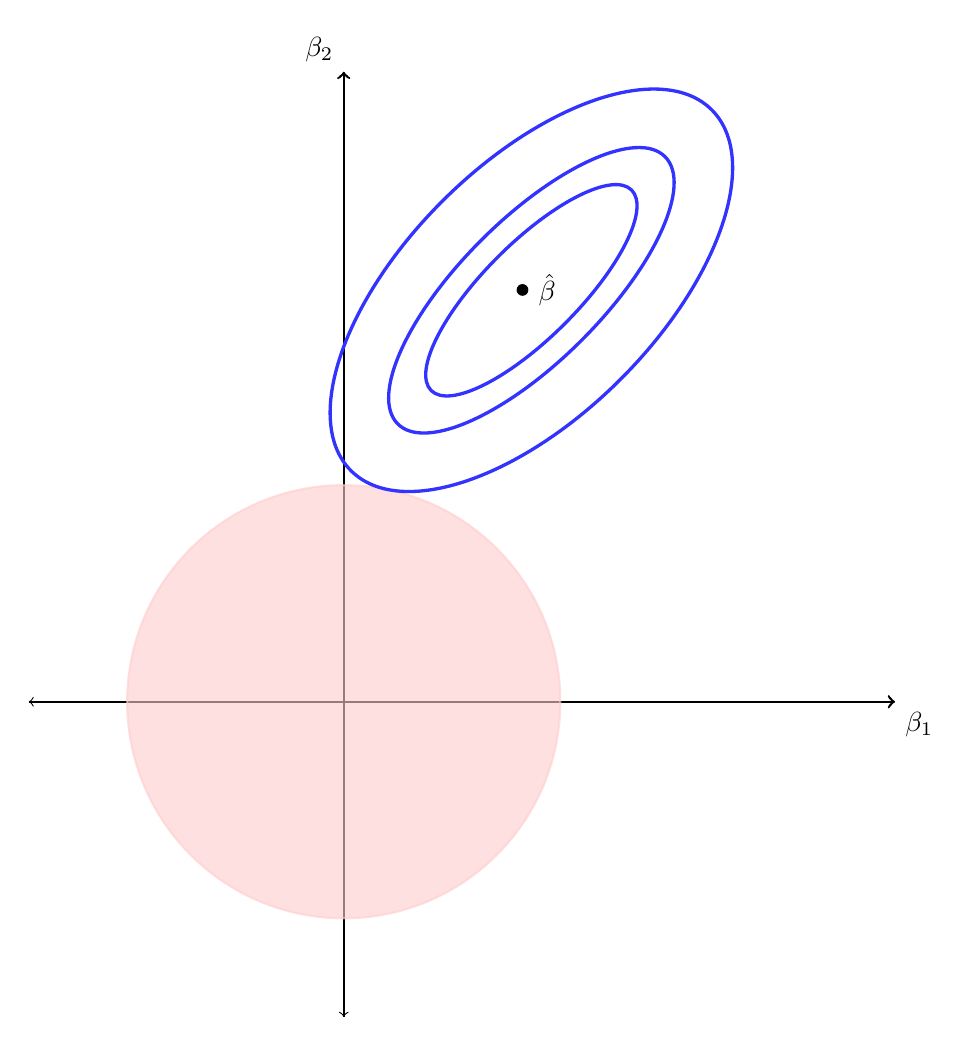
\begin{tikzpicture}
\draw[<->] (-4,0) -- (7,0) coordinate (x axis);
\draw[<->] (0,-4.0) -- (0,8.0) coordinate (y axis);
\draw[thick,->] (-4,0) -- (7,0) node[anchor=north west] {$\beta_1$};
\draw[thick,->] (0,-4) -- (0,8) node[anchor=south east] {$\beta_2$};

\draw[red!20, thick, fill, opacity=0.6] (0,0) circle (2.75cm);

\draw[very thick, blue!80, rotate=45] (5.38,2.01) ellipse (3.24cm and 1.6cm);
\draw[very thick, blue!80, rotate=45] (5.38,2.01) ellipse (2.4cm and 0.9cm);
\draw[very thick, blue!80, rotate=45] (5.38,2.01) ellipse (1.8cm and 0.60cm);

\node at (2.27,5.23)[circle,fill,inner sep=1.5pt, label=right:$\hat{\beta}$]{};
\end{tikzpicture}

}}\hspace{1.5cm}
\subfloat[Lasso constraint region, $\left|\beta_{1} \right| + \left|\beta_{2} \right| \leq t $]{\scalebox{0.6}{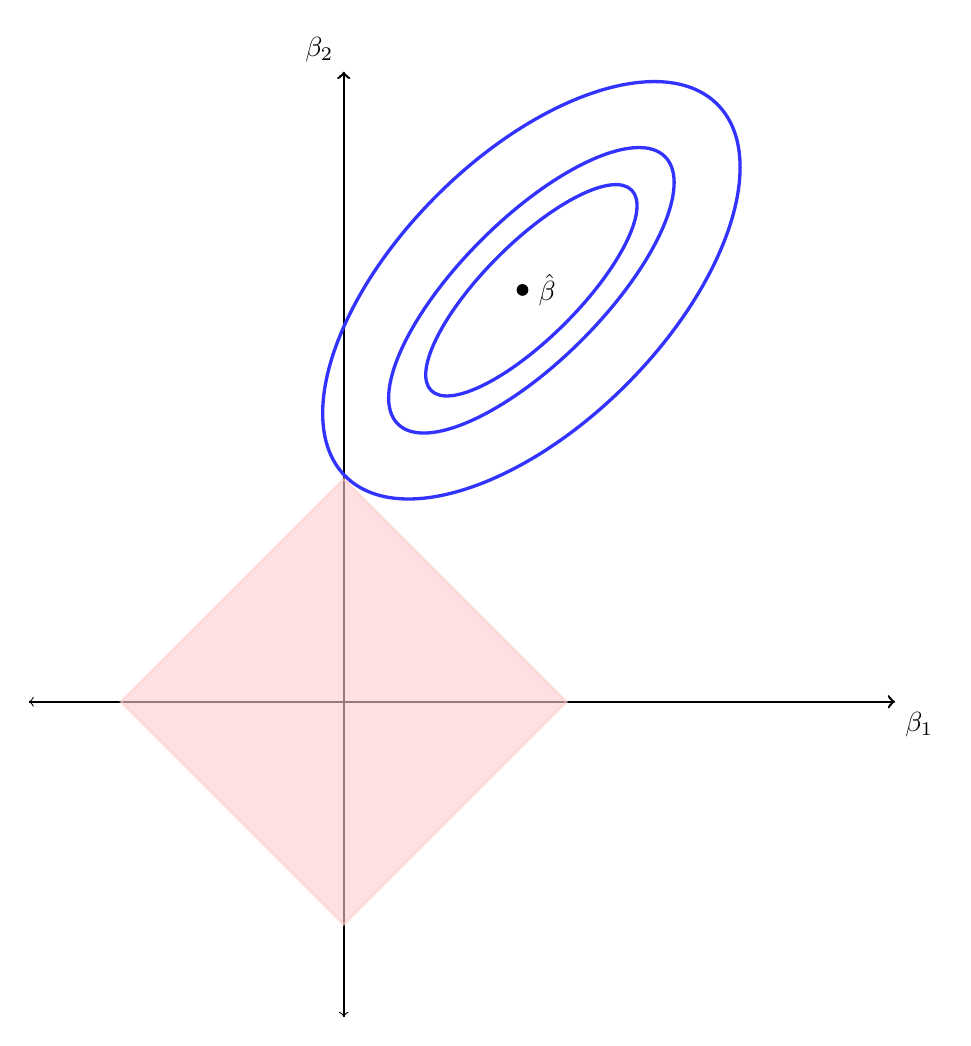
\begin{tikzpicture}
\draw[<->] (-4,0) -- (7,0) coordinate (x axis);
\draw[<->] (0,-4.0) -- (0,8.0) coordinate (y axis);
\draw[thick,->] (-4,0) -- (7,0) node[anchor=north west] {$\beta_1$};
\draw[thick,->] (0,-4) -- (0,8) node[anchor=south east] {$\beta_2$};

\draw[red!20, thick, fill, opacity=0.6, rotate=45] (-2,-2) rectangle (2,2);

\draw[very thick, blue!80, rotate=45] (5.38,2.01) ellipse (3.34cm and 1.7cm);
\draw[very thick, blue!80, rotate=45] (5.38,2.01) ellipse (2.4cm and 0.9cm);
\draw[very thick, blue!80, rotate=45] (5.38,2.01) ellipse (1.8cm and 0.60cm);

\node at (2.27,5.23)[circle,fill,inner sep=1.5pt, label=right:$\hat{\beta}$]{};
\end{tikzpicture}}}
\caption[RSS contours and constraint regions for ridge and lasso]{We depict the contours of the minimized RSS with added shrinkage penalty (blue) and the constraint regions (red) for ridge and lasso, respectively. Replicated figure from \cite{hastie2008elements}.}
\label{fig:ridgelassoconstraint}
\end{figure}

\begin{figure}[H]
  \centering
    \scalebox{0.8}{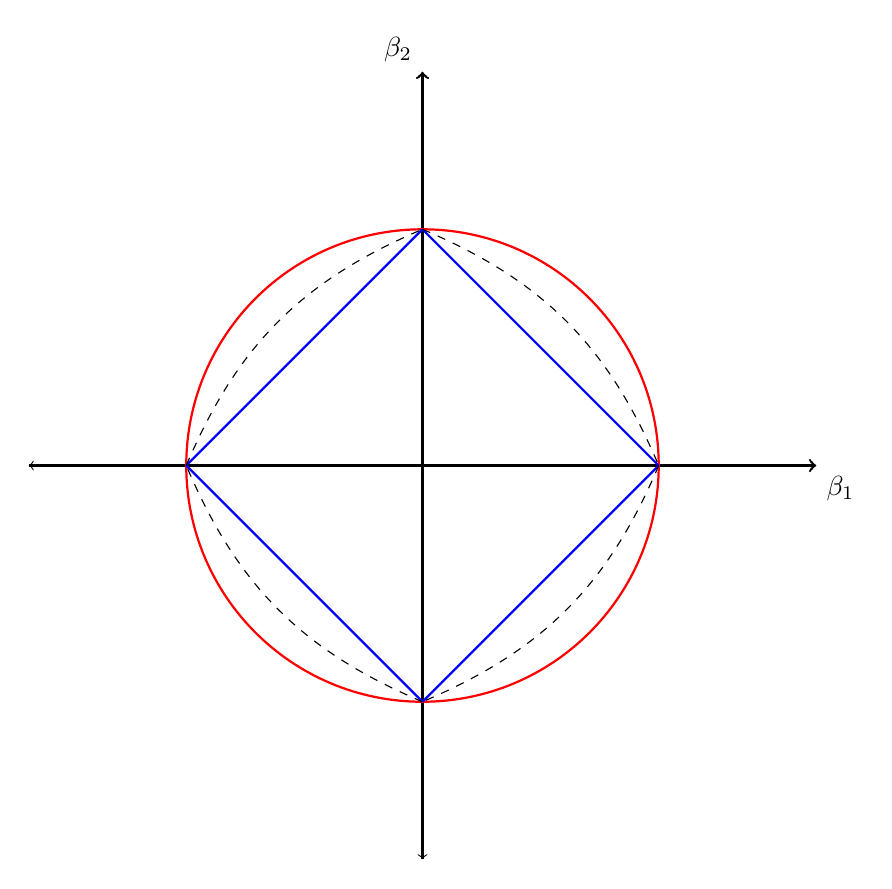
\begin{tikzpicture}
\draw[<->] (-5,0) -- (5,0) coordinate (x axis);
\draw[<->] (0,-5.0) -- (0,5.0) coordinate (y axis);
\draw[thick,->] (-5,0) -- (5,0) node[anchor=north west] {$\beta_1$};
\draw[thick,->] (0,-5) -- (0,5) node[anchor=south east] {$\beta_2$};
\draw[red, thick] (0,0) circle (3 cm);
\draw[blue,thick,-] (0,3) -- (3,0);
\draw[blue,thick,-] (-3,0) -- (0,3);
\draw[blue,thick,-] (-3,0) -- (0,-3);
\draw[blue,thick,-] (3,0) -- (0,-3);
\draw [dashed] (-3,0) to [bend left=22] (0,3);
\draw [dashed] (0,3) to [bend left=22] (3,0);
\draw [dashed] (3,0) to [bend left=22] (0,-3);
\draw [dashed] (0,-3) to [bend left=22] (-3,0);
\end{tikzpicture}


}
    \caption[Constraint regions for ridge, lasso, and elastic net]{This graph compares the constraint regions of all three regularization methods: ridge (red), lasso (blue), and elastic net (dashed black). Replicated figure from \cite{zou2005regularization}.}
    \label{fig:plotnorms}
\end{figure}

\begin{figure}[H]
        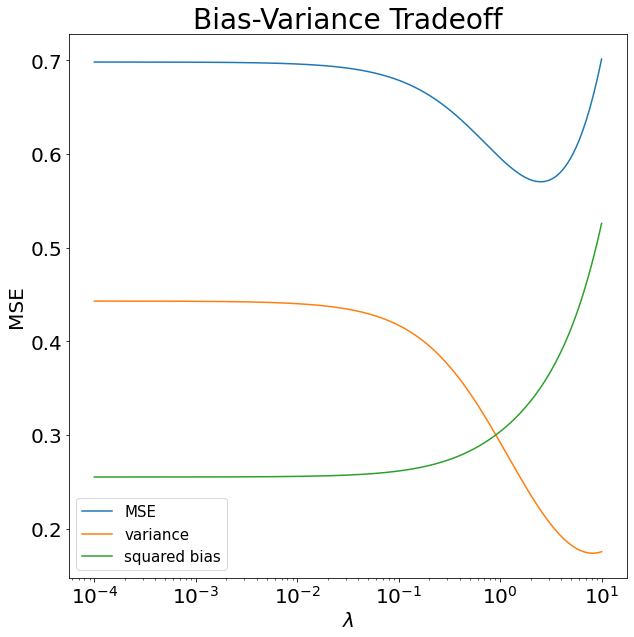
\includegraphics[scale=0.45]{material/Img/bias_var_tradeoff.png}%\hspace{-1.2cm}
        \centering
        \caption[Decomposition of bias-variance trade-off]{We depict the bias-variance trade-off with the test MSE (blue), variance (orange), and squared bias (green) of a ridge simulation from Case 2 in Section \ref{section:msesim}.}
        \label{fig:bias_var}
    \end{figure}

\begin{figure}[H]
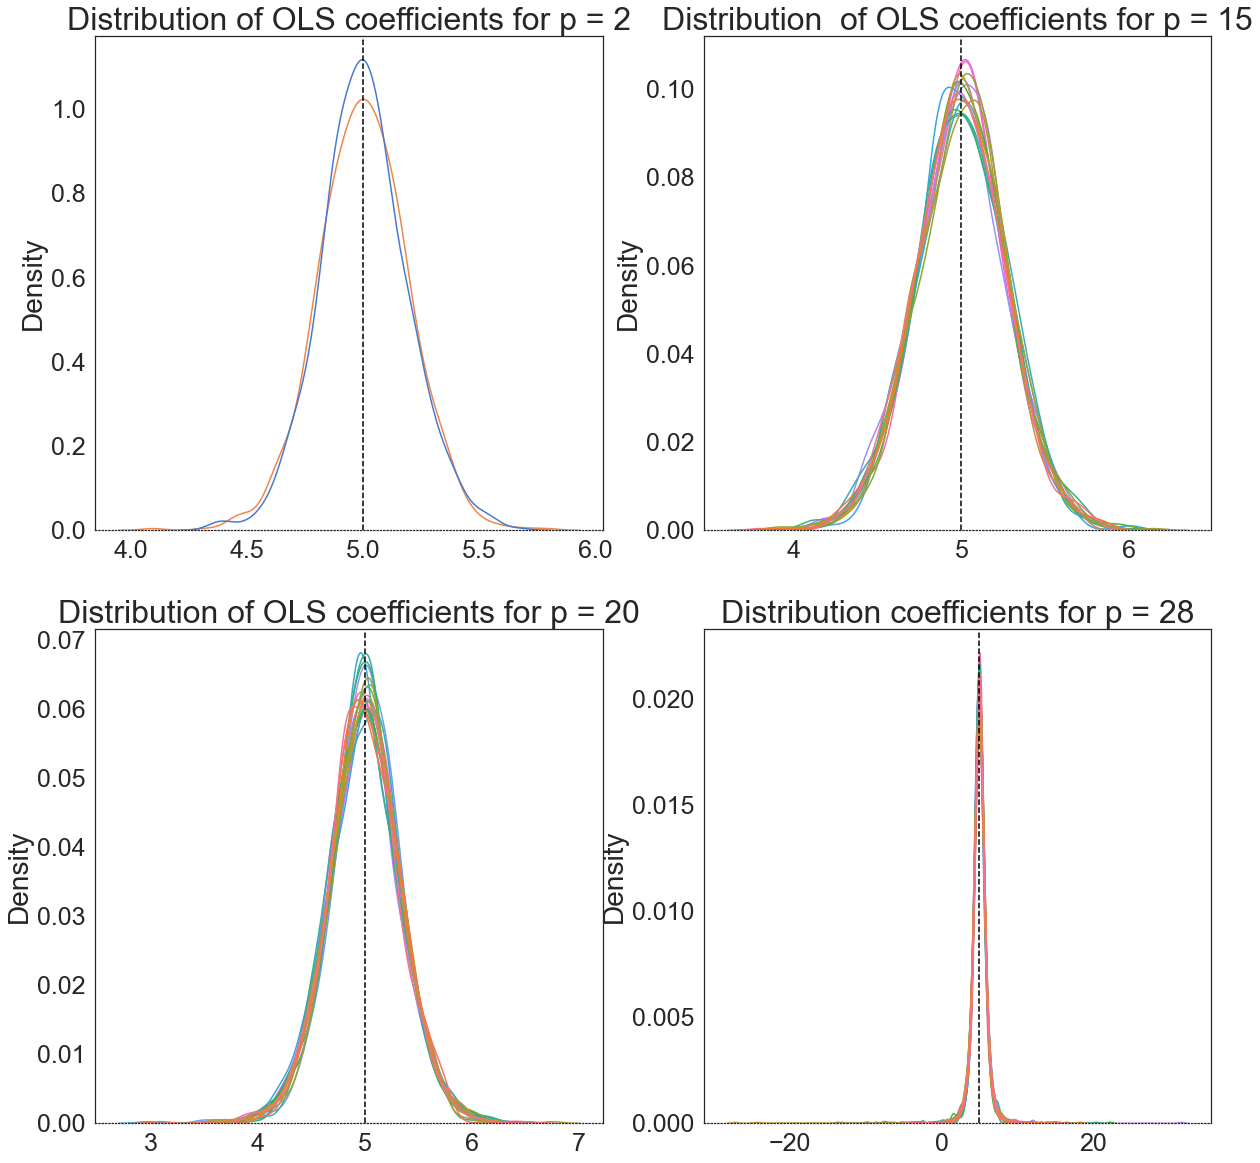
\includegraphics[scale=0.3]{material/Img/ols_distr.png}
\centering
\caption[Distribution of OLS coefficients]{Each quadrant represents the simulated distributions of OLS coefficients for a different number of regressors $p\in \{2,15,20,28\}$. The sample size ($n = 30$) and the total number of drawn samples (1000) remain the same for each case. The dashed vertical lines indicate the size of the true beta coefficients set to $5$.}
\label{fig:old_distr}
\end{figure}

\begin{figure}[H]
    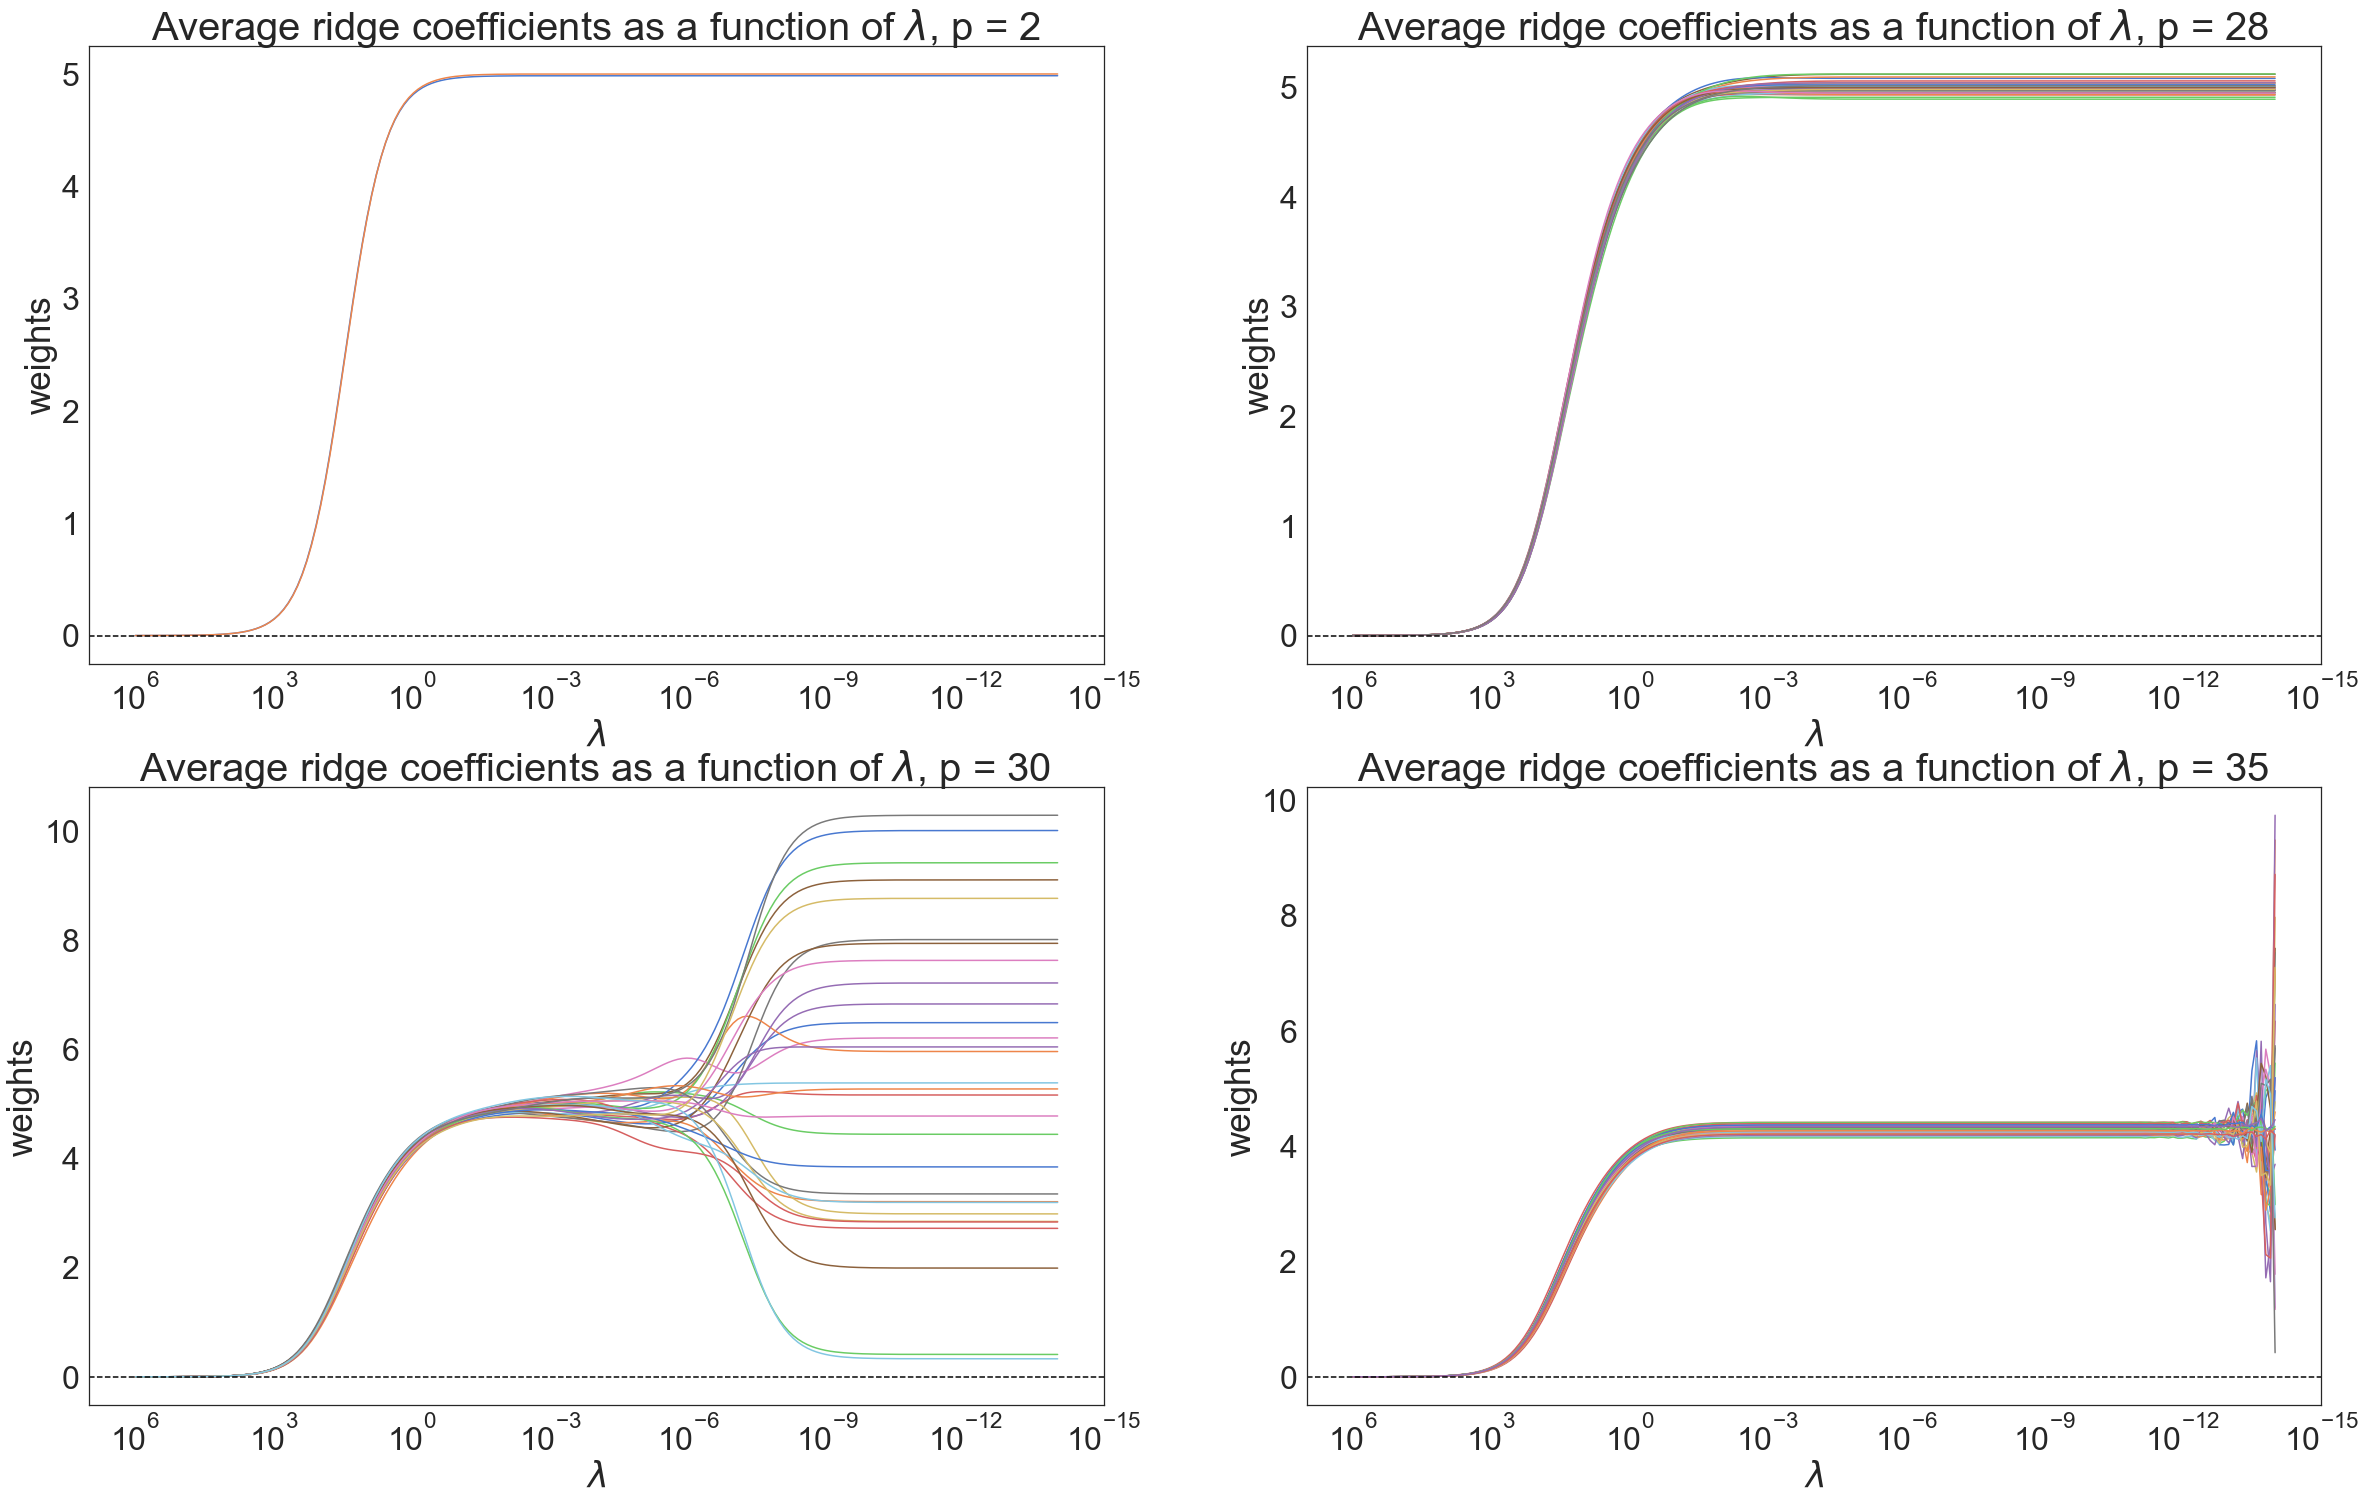
\includegraphics[scale=0.2]{material/Img/average_ridge_plot_betas.png}
    \centering
    \caption[Average ridge coefficients as a function o$\lambda$]{The average ridge coefficients as a function o$\lambda$ is represented for different values of $p\in \{2,28,30,35\}$, where the sample size ($n=30$) remains constant. The true beta coefficients are set equal to $5$ and the total number of simulated iterations for each case is $500$.}
\label{fig:avg_ridge_betas}
\end{figure}
    
\begin{figure}[H]
        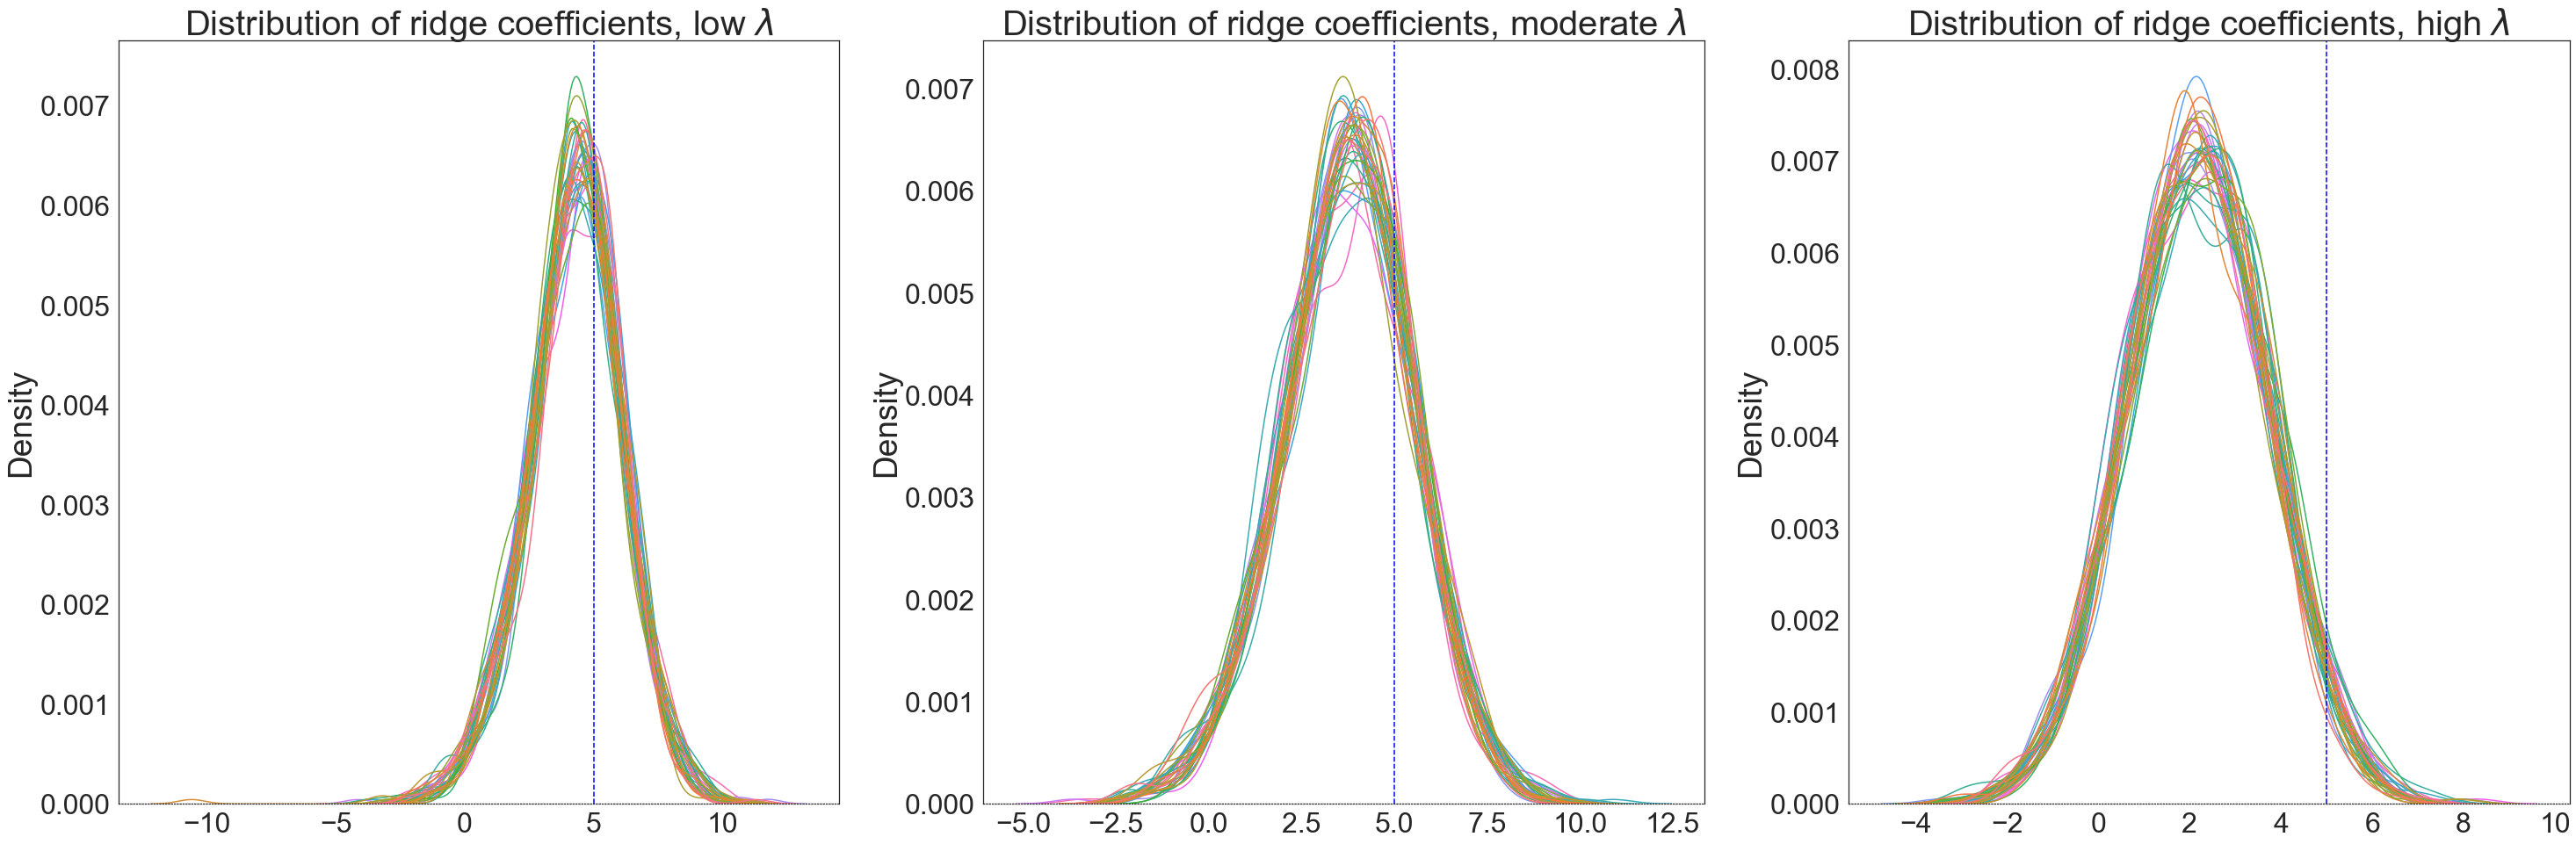
\includegraphics[scale=0.17]{material/Img/ridge_shrunken_beta_dist_35.png}
        \centering
        \caption[Distribution of ridge coefficients]{The distributions of ridge coefficients for low (left), moderate (center), and high (right) values of $\lambda$ are represented above. The dashed vertical lines indicate the true betas set equal to $5$. The number of observations ($n=30$), regressors ($p = 35$) and simulated draws ($500$) remain constant.}
\label{fig:ridge_shrunken_betas}
\end{figure}

\begin{figure}[H]
        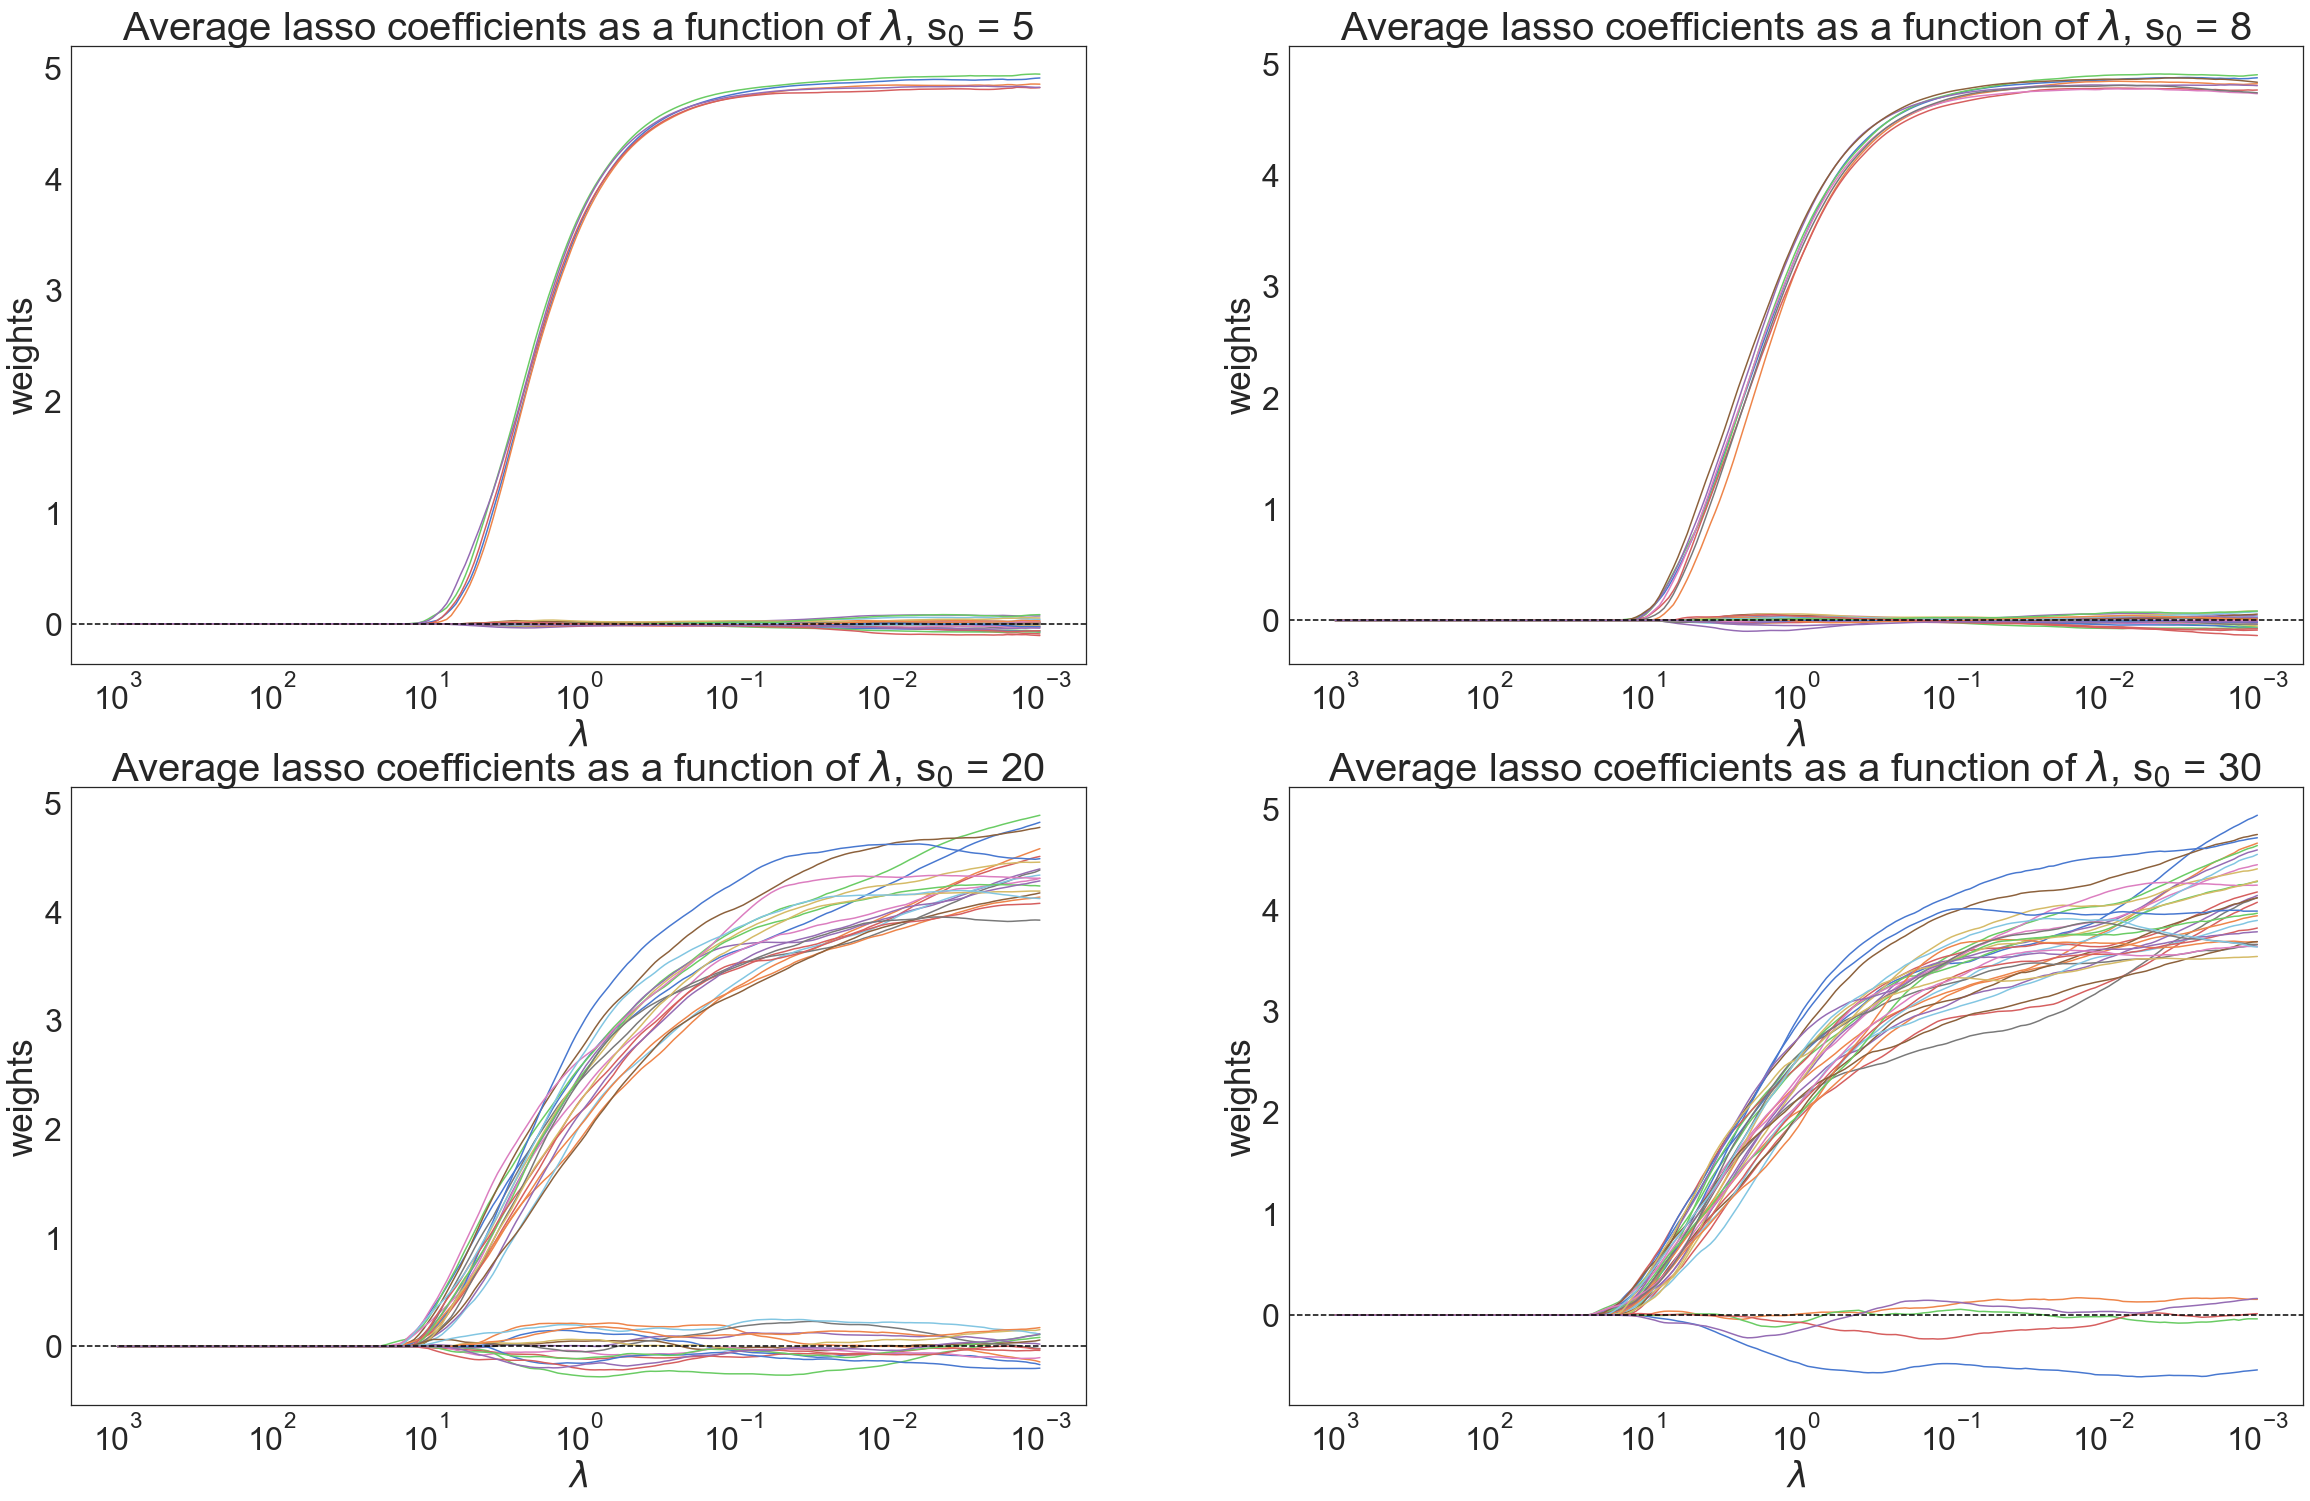
\includegraphics[scale=0.2]{material/Img/average_lasso_plot_betas.png}
        \centering
        \caption[Average lasso coefficients as a function of $\lambda$]{The average lasso coefficients as a function of $\lambda$ are depicted, where $n=30$ and $p=35$, for varying degrees of sparsity. All truly non-zero beta coefficients have a magnitude of $5$. The total number of simulated iterations is $100$ for each case.}
\label{fig:avg_lasso_betas}
\end{figure}
    
\begin{figure}[H]
        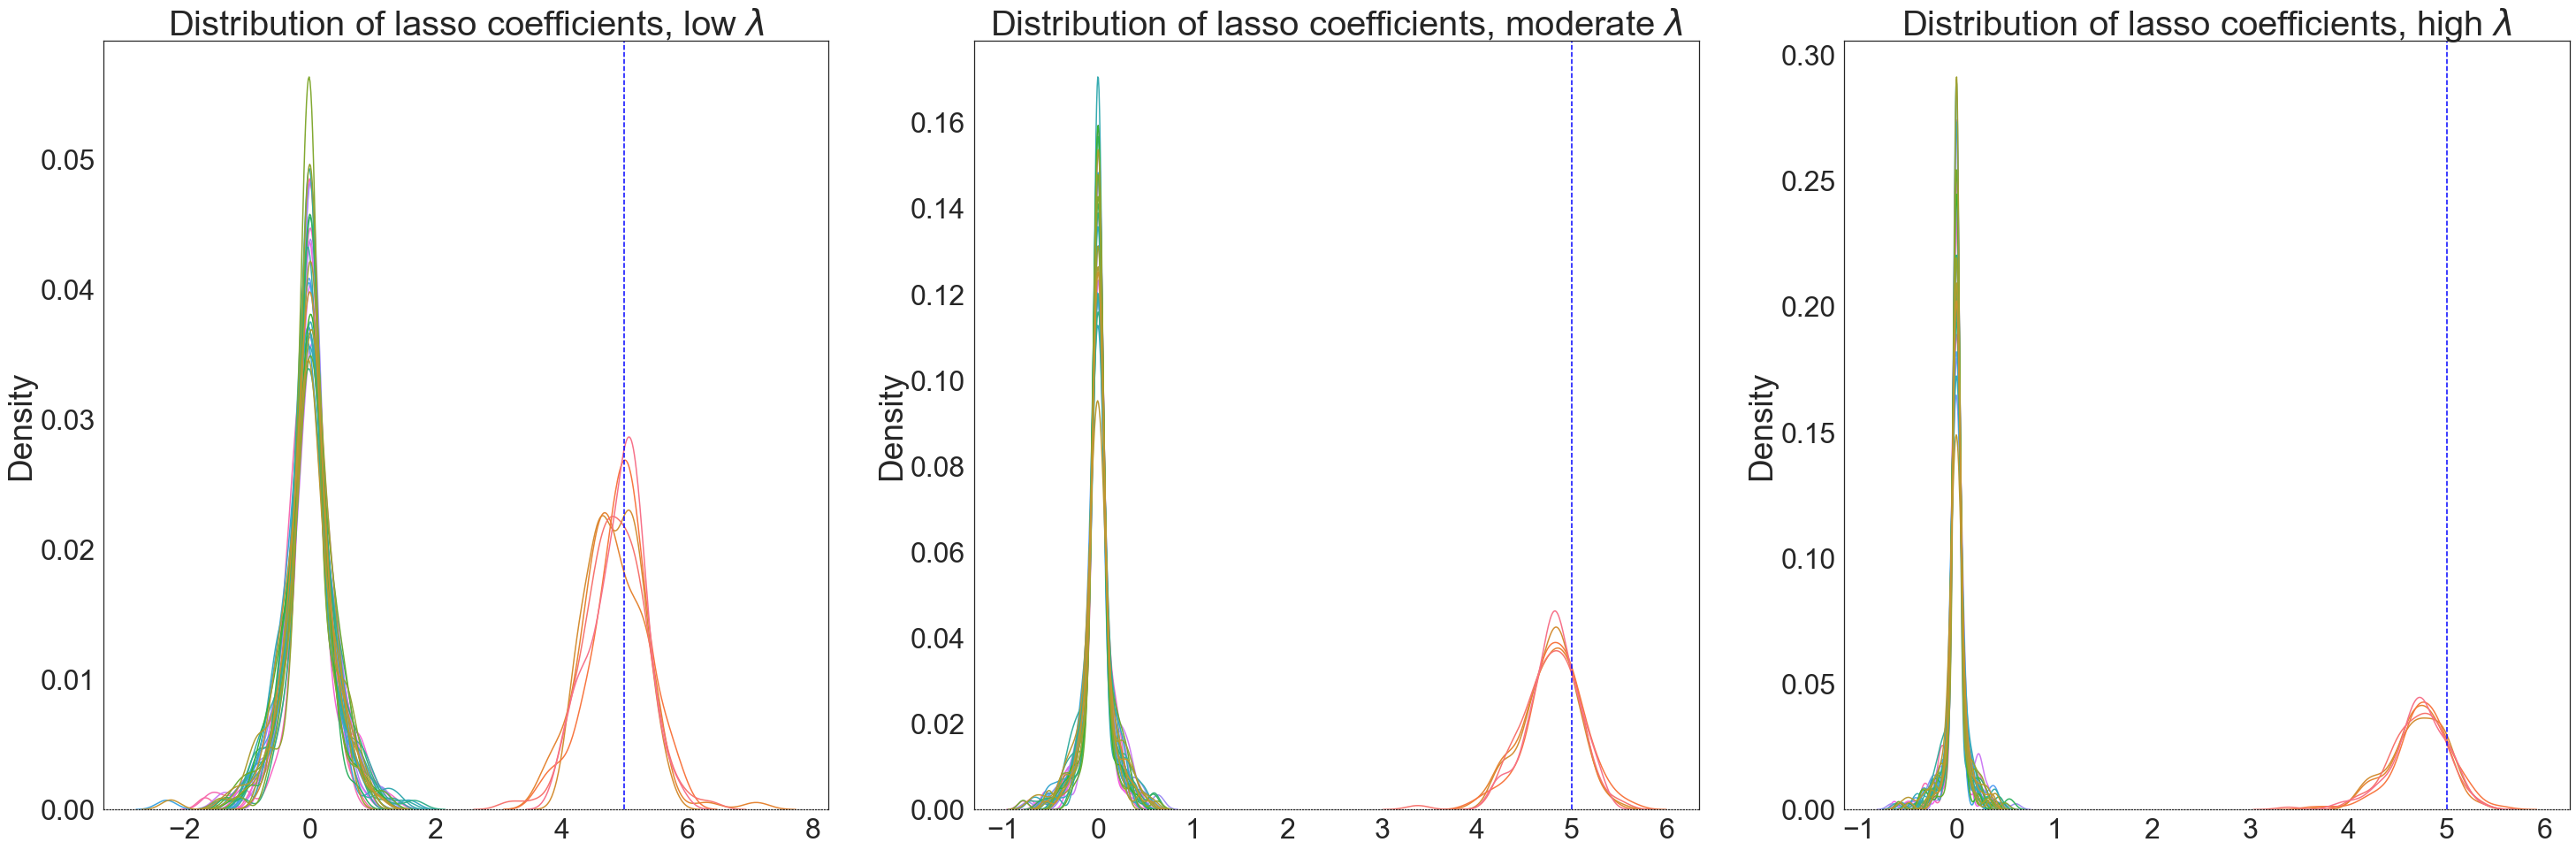
\includegraphics[scale=0.17]{material/Img/lasso_shrunken_beta_dist_35.png}
        \centering
        \caption[Distribution of lasso coefficients]{The distributions of lasso coefficients for low (left), moderate (center), and high (right) value of $\lambda$ are represented above. The dashed vertical lines indicate the true size of the non-zero beta coefficients, which are set equal to $5$. The number of observations ($n=30$), regressors ($p=35$), and simulate draws (100) remain constant for each case.}
\label{fig:lasso_shrunken_betas}
\end{figure}

\begin{figure}[H]
        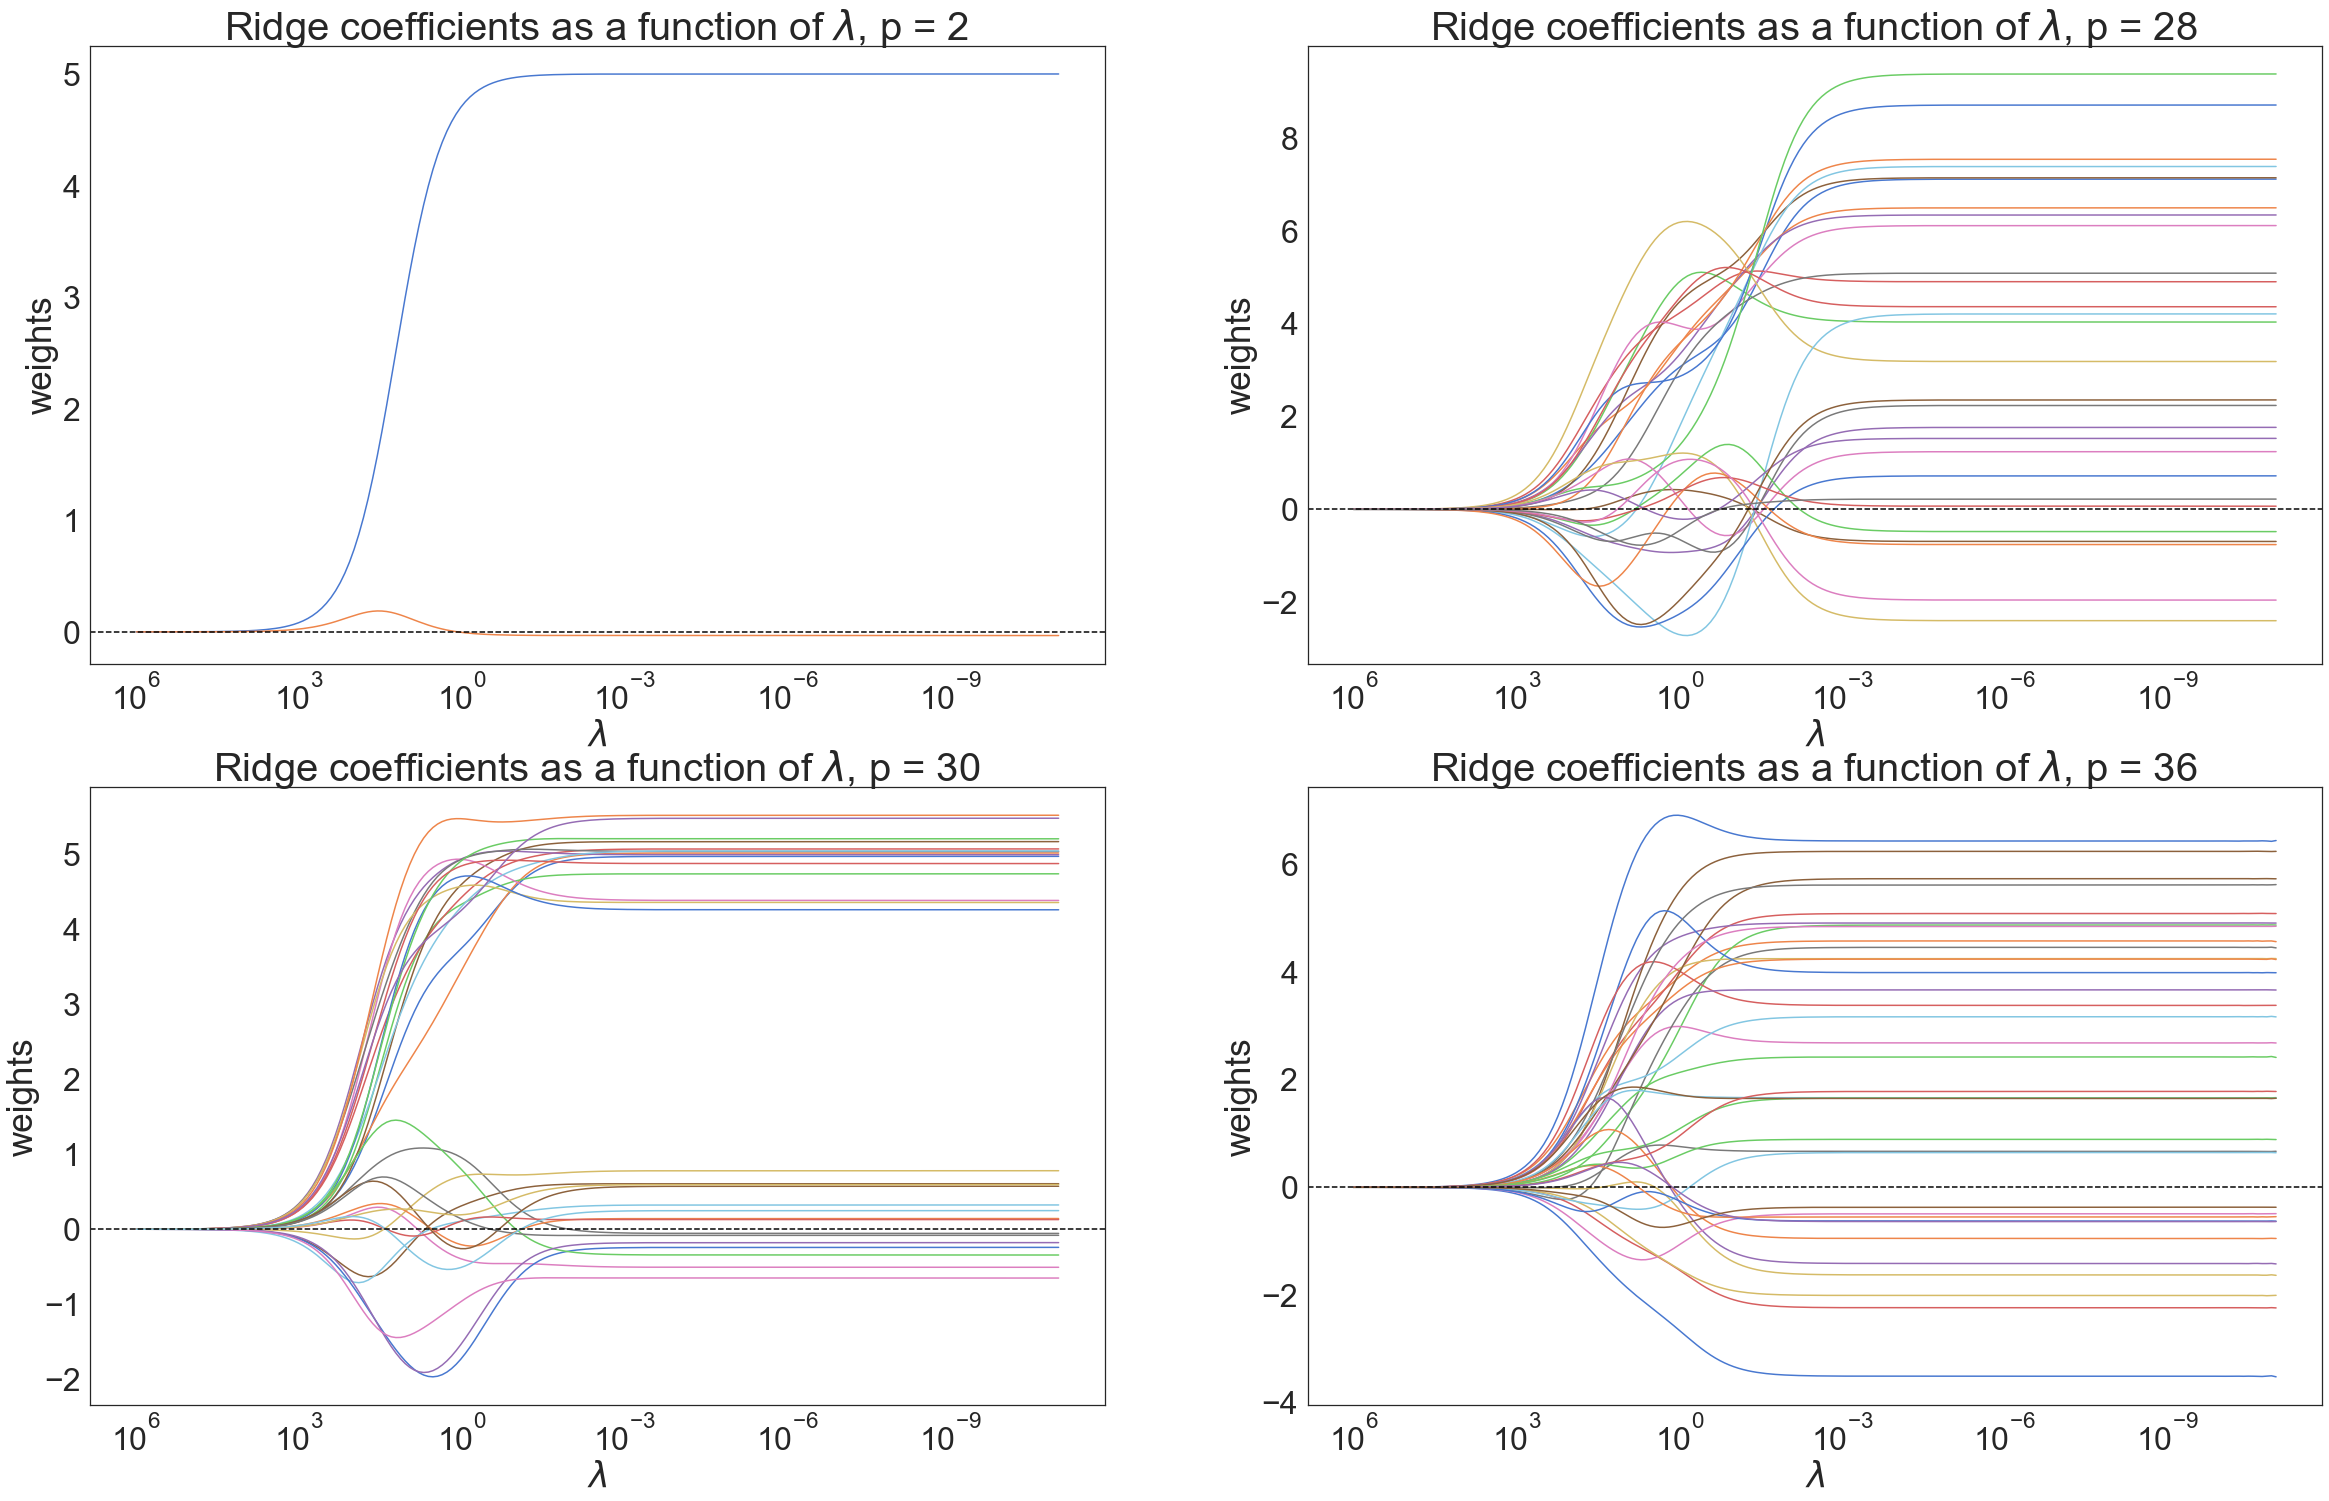
\includegraphics[scale=0.20]{material/Img/ridge_plot_betas.png}
        \centering
        \caption[Ridge coefficients as a function of $\lambda$ for a single sample]{The ridge coefficients as a function of $\lambda$ for a single sample for different values of $ p\in \{2,28,30,36\}$ are depicted above. The number of observations ($n=30$) remains constant for each case. Half of the true beta coefficients are set equal to $5$, while the remaining are set to $0$.}
        \label{fig:ridge_single_sample}
\end{figure}

\begin{figure}[H]
        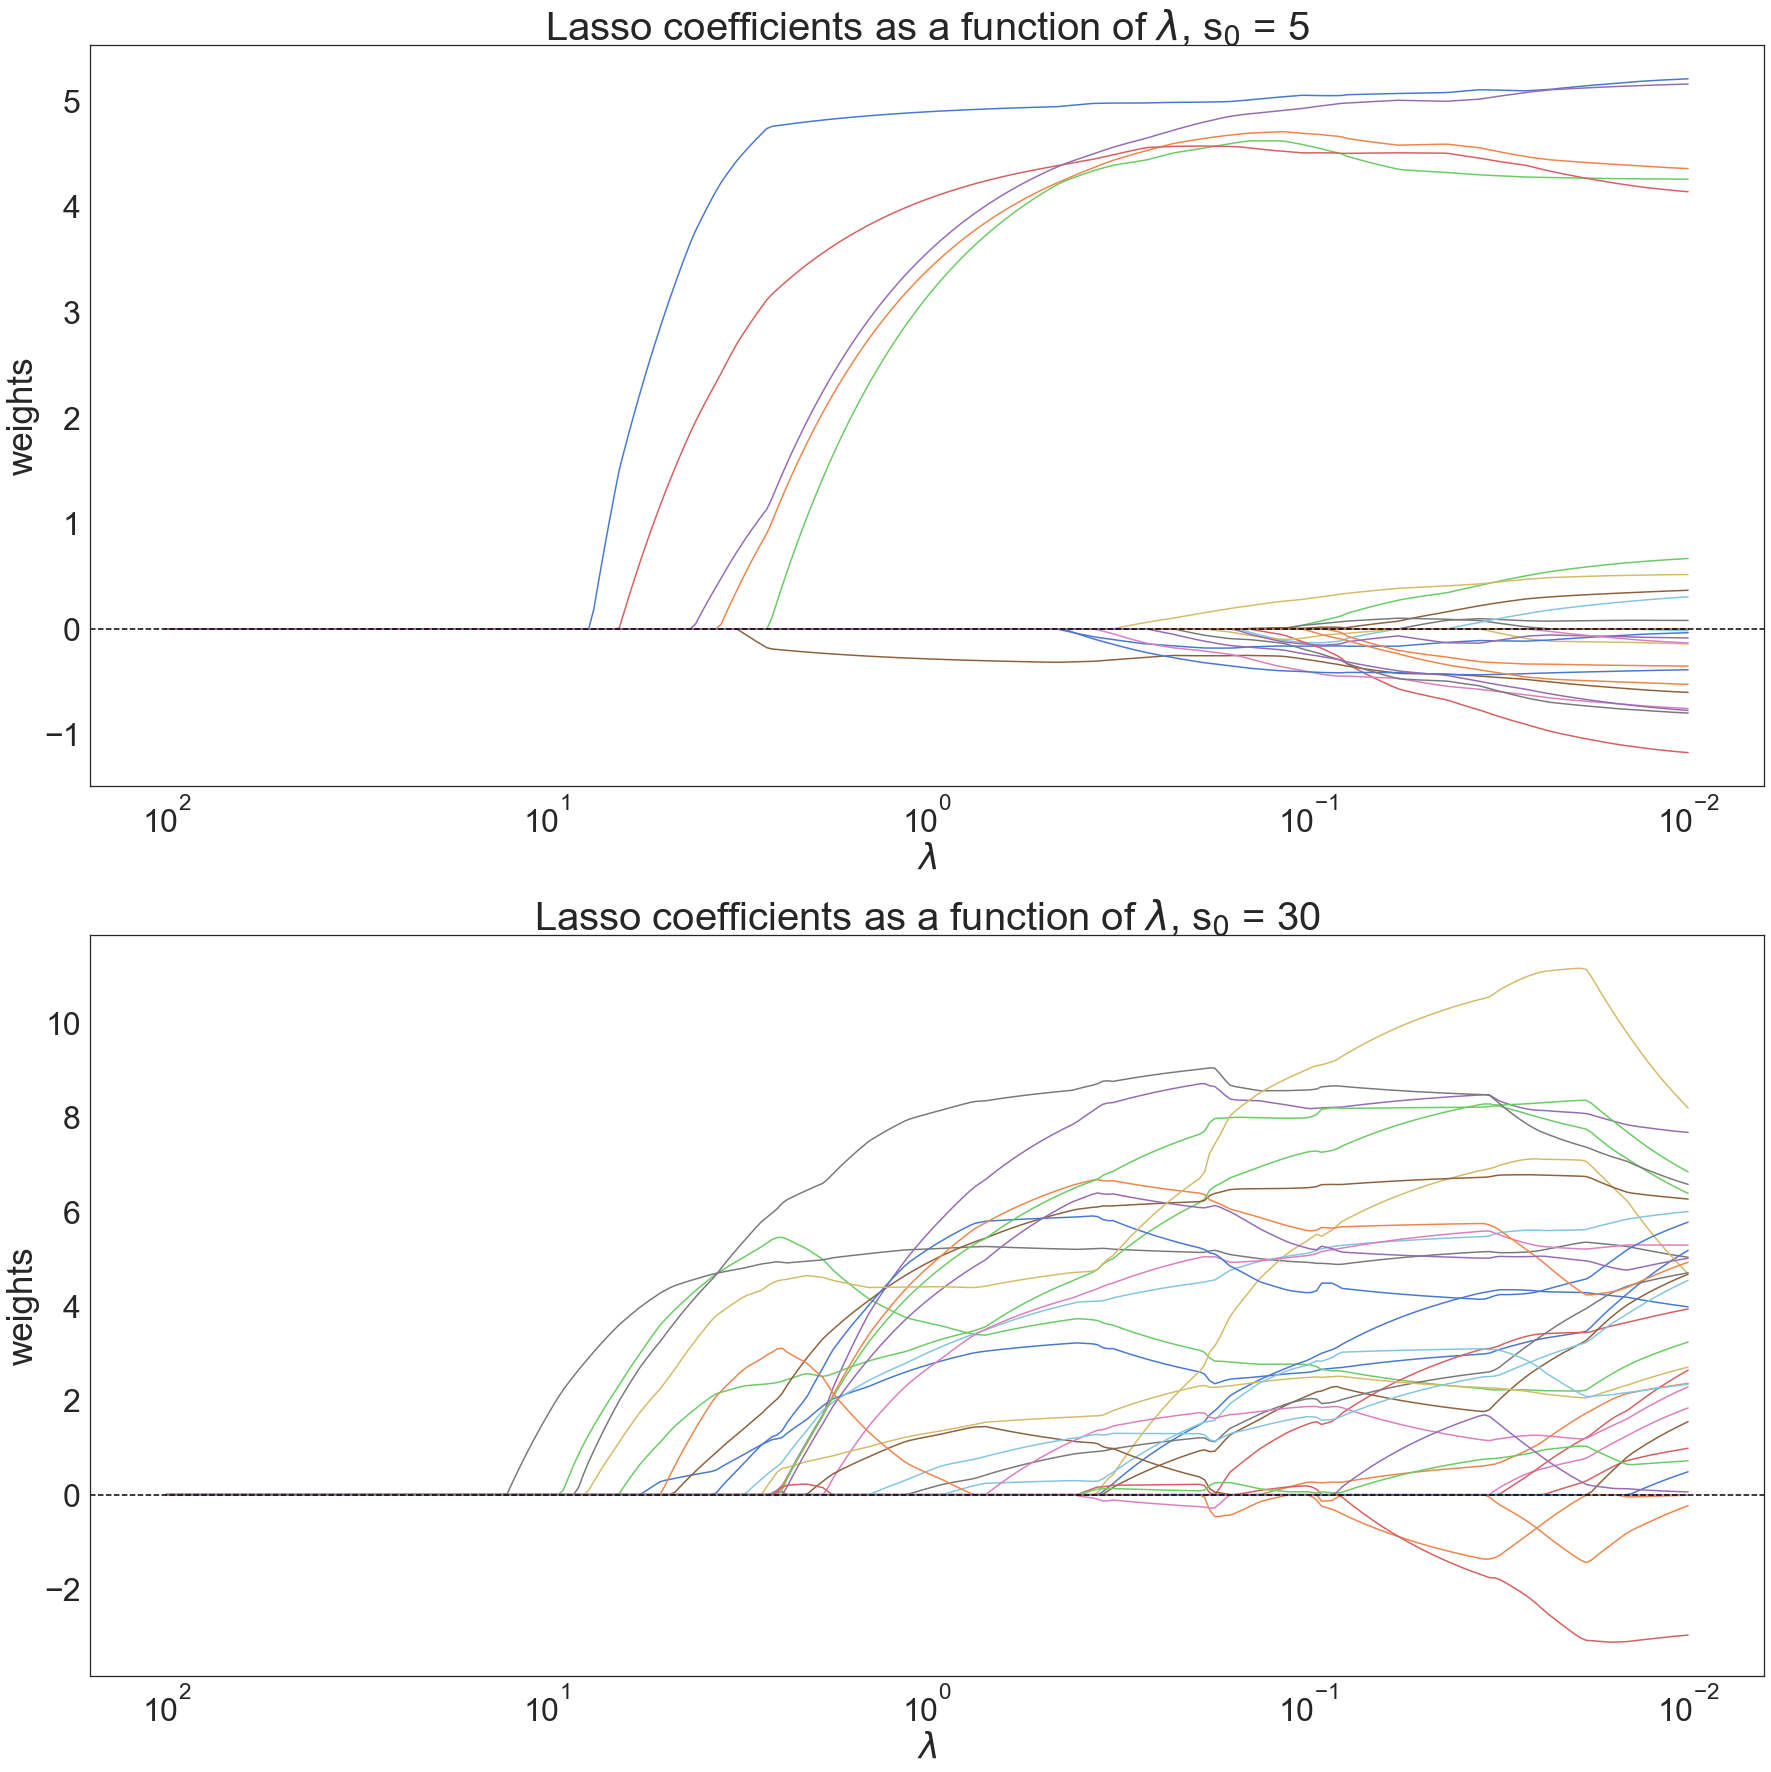
\includegraphics[scale=0.2]{material/Img/lasso_plot_betas.png}
        \centering
        \caption[Lasso coefficients as a function of $\lambda$ for a single sample draw]{The lasso coefficients as a function of $\lambda$ for a single sample draw with varying degrees of sparsity is depicted above. The top graph represents a case of high sparsity, where the sparsity index is $s_{0}=5$, while the lower graph corresponds to a case of low sparsity with a sparsity index of $s_{0}=30$.}  
        \label{fig:lasso_single_sample}
\end{figure}
    
\begin{figure}[H]
        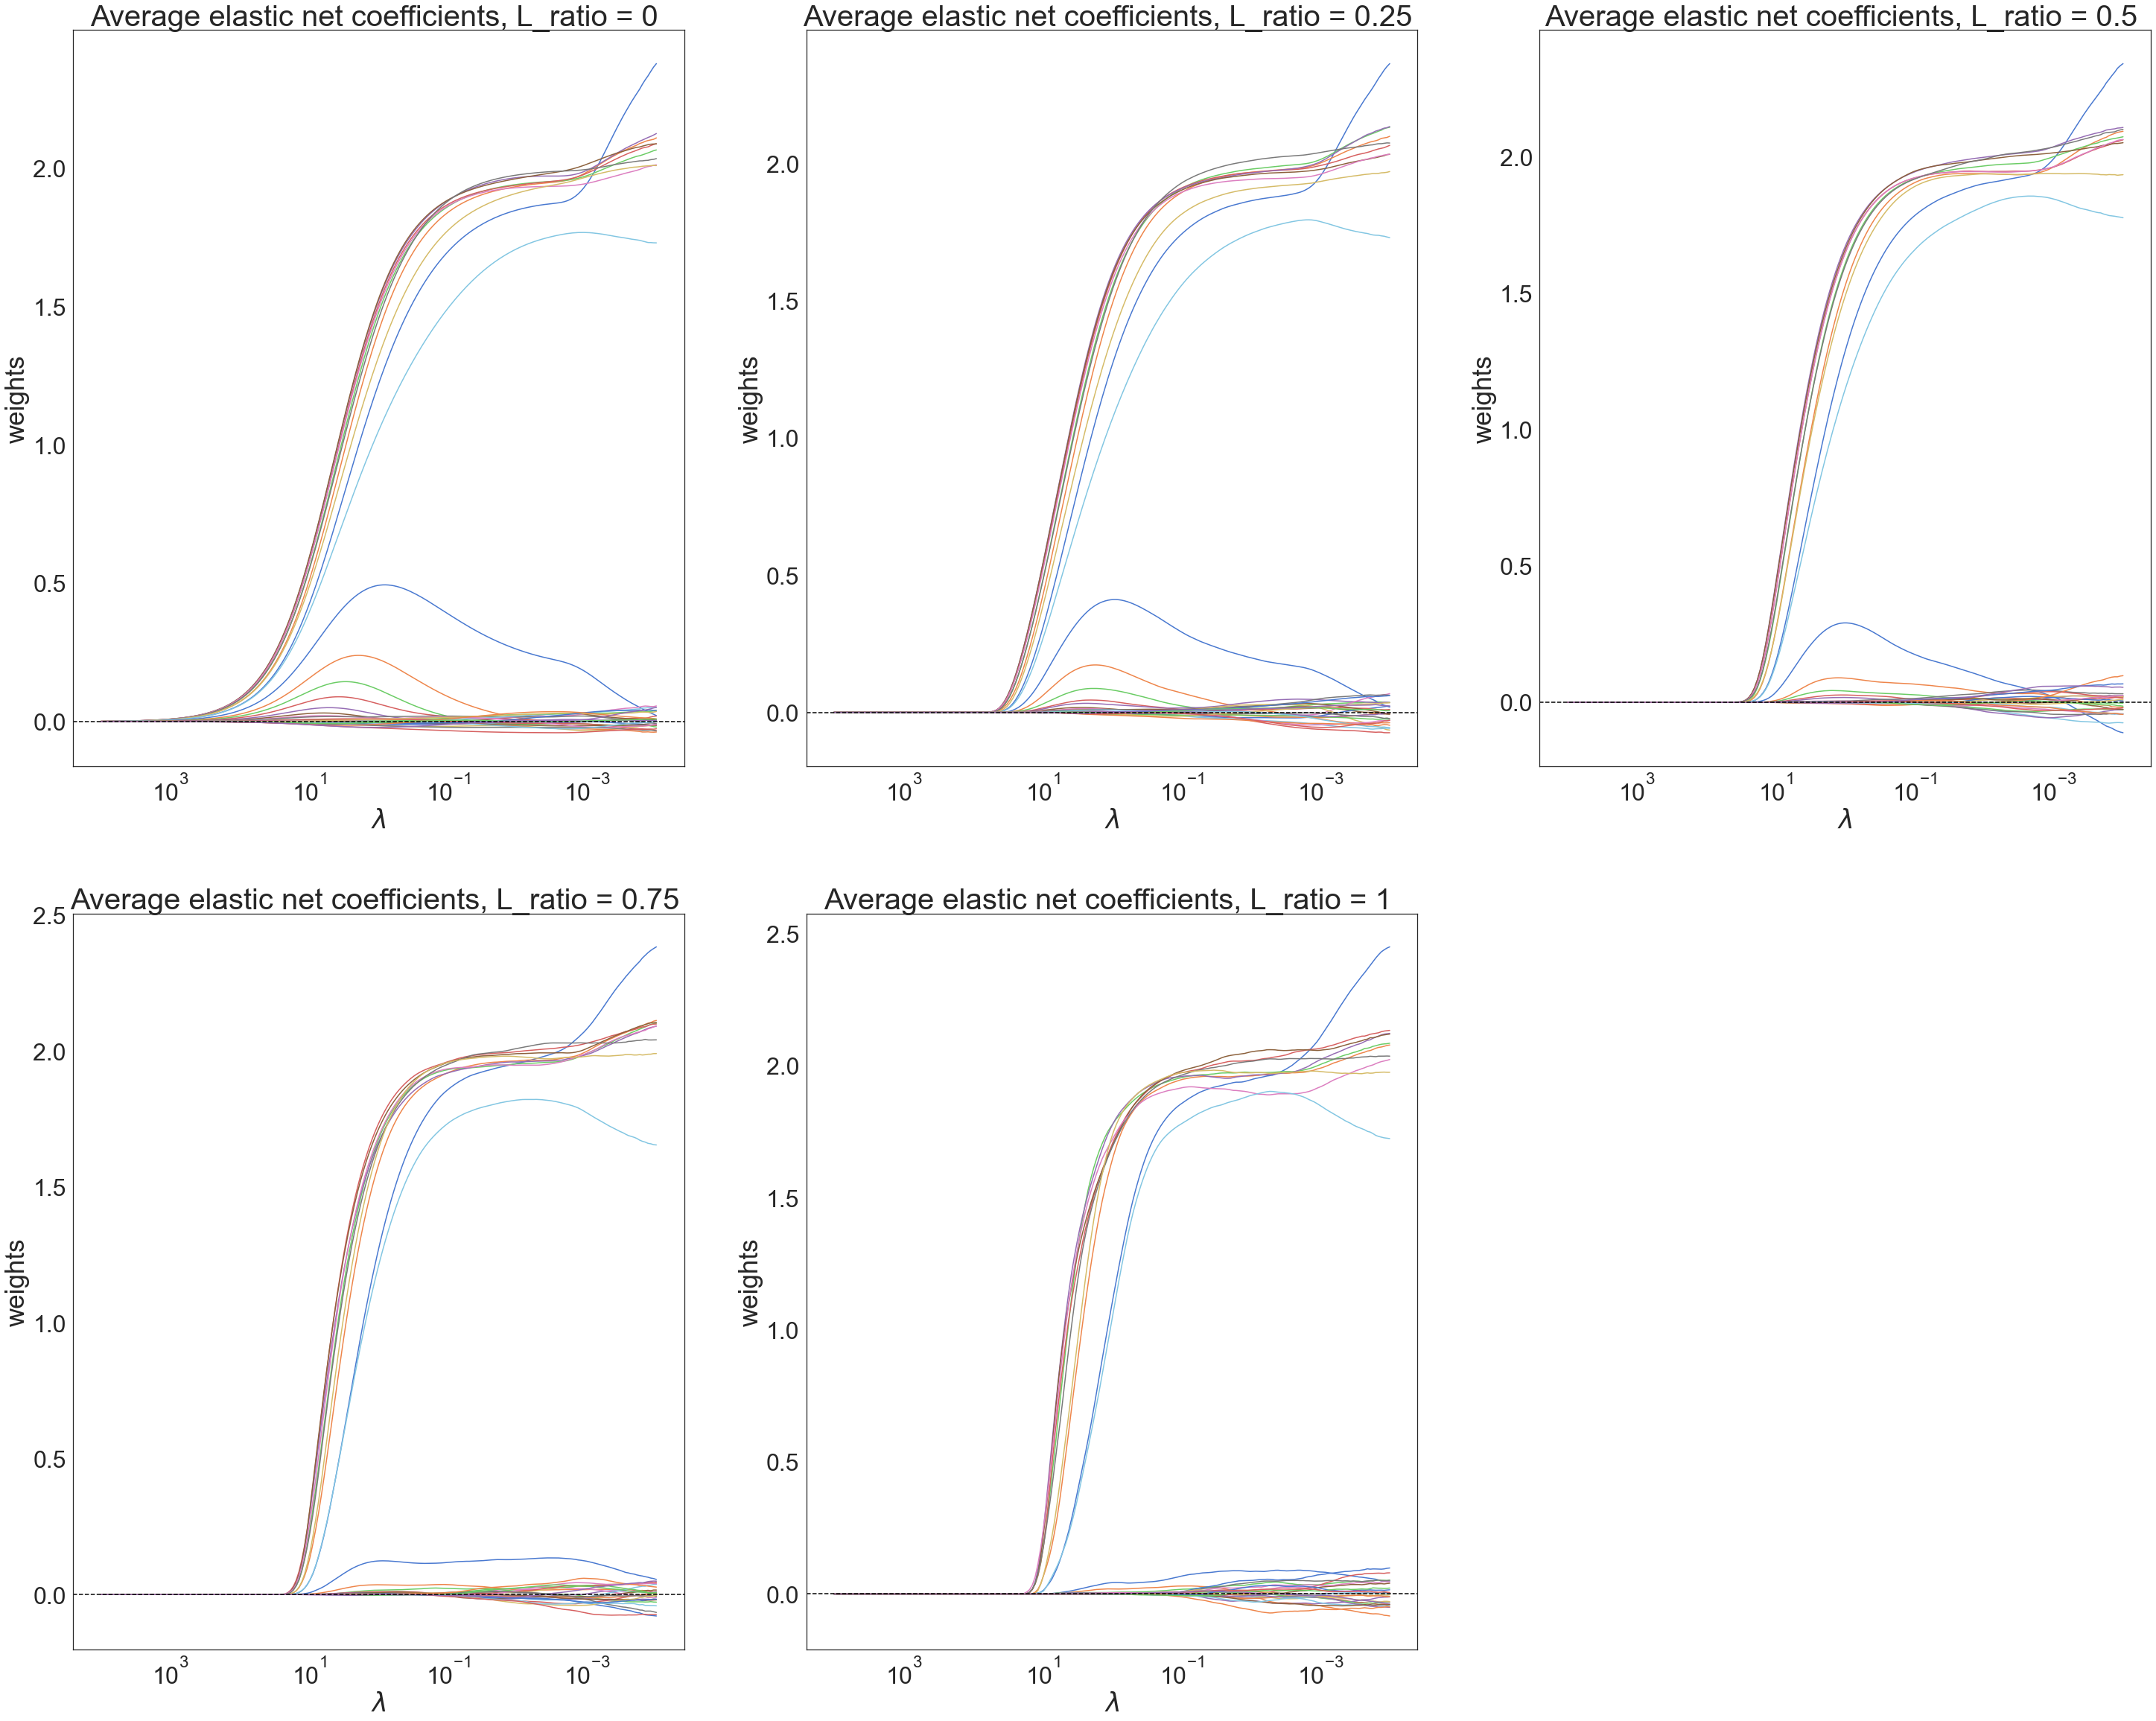
\includegraphics[scale=0.17]{material/Img/elastic_net_plot_average_betas.png}
        \centering
        \caption[Average naive elastic net coefficient estimates]{The average naive elastic net coefficient estimates as a function of $\lambda$ for different $\ell_1$-ratio are represented above. The number of observations ($n=30$), regressors ($p=35$), simulations ($500$), and the pairwise correlation factor ($0.7$) remain constant for each case. We set $25$ true beta coefficients to $2$, while the remaining $10$ beta coefficients are set equal to $0$.}
        \label{fig:elnet_avg_betas}
\end{figure}
    
\begin{figure}[H]
        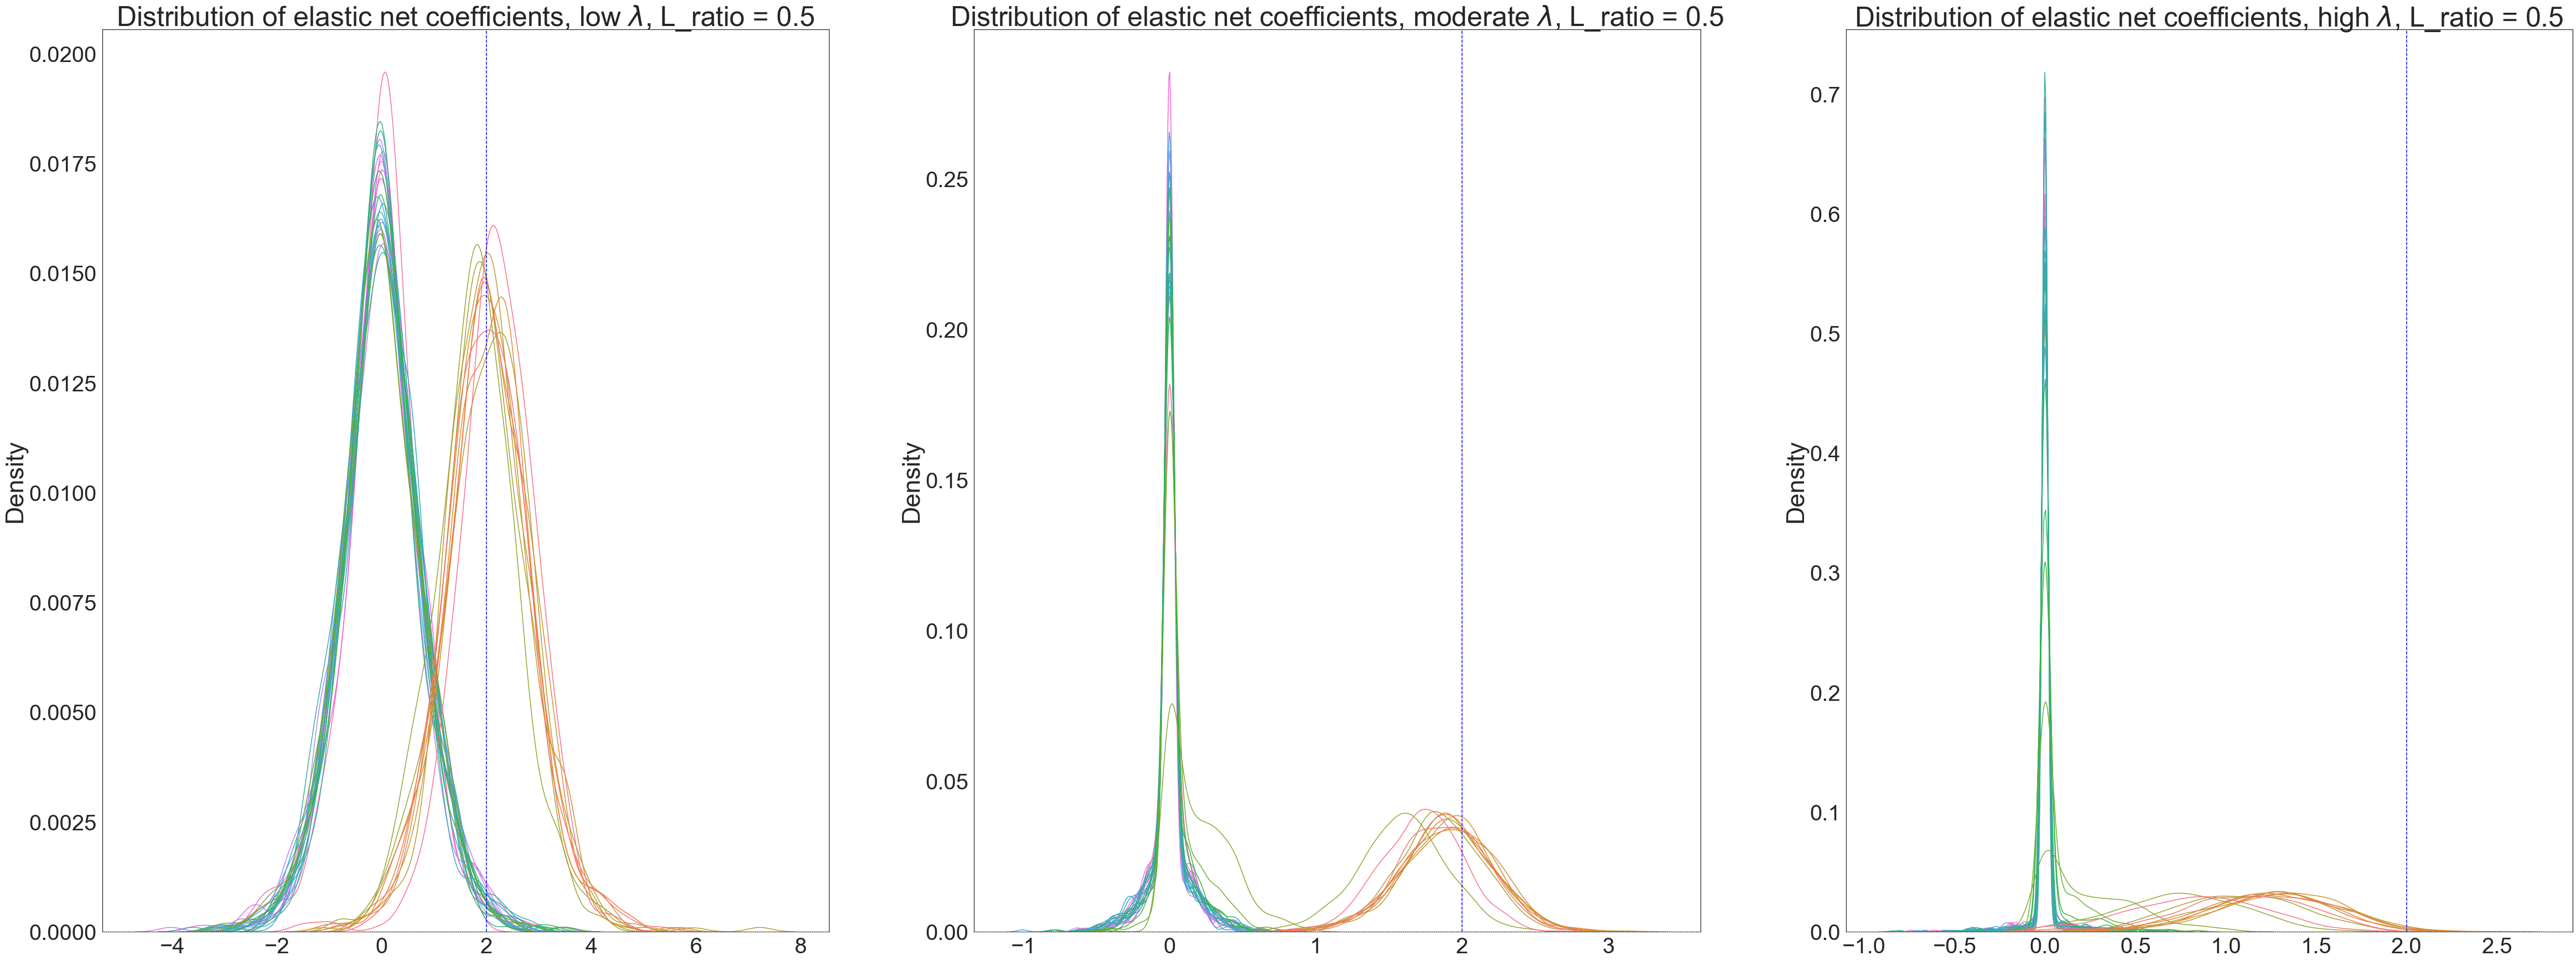
\includegraphics[scale=0.11]{material/Img/elastic_net_shrunken_beta_dist_35_0.5.png}
        \centering
        \caption[Distribution of naive elastic net coefficients]{The distributions of the naive elastic net ($\ell_1$-ratio$ = 0.5$) coefficients for low (left), moderate (center), and high (right) values of $\lambda$ is represented above. The dashed vertical line indicates the size of the true beta coefficients, which are set equal to $2$, while all remaining true beta coefficients are set equal to $0$. The number of observations ($n=30$), regressors ($p=35$), and simulated iterations ($100$) remain constant for each case.}
\label{fig:elnet_shrunken_betas}
\end{figure}
    
\begin{figure}[H]
        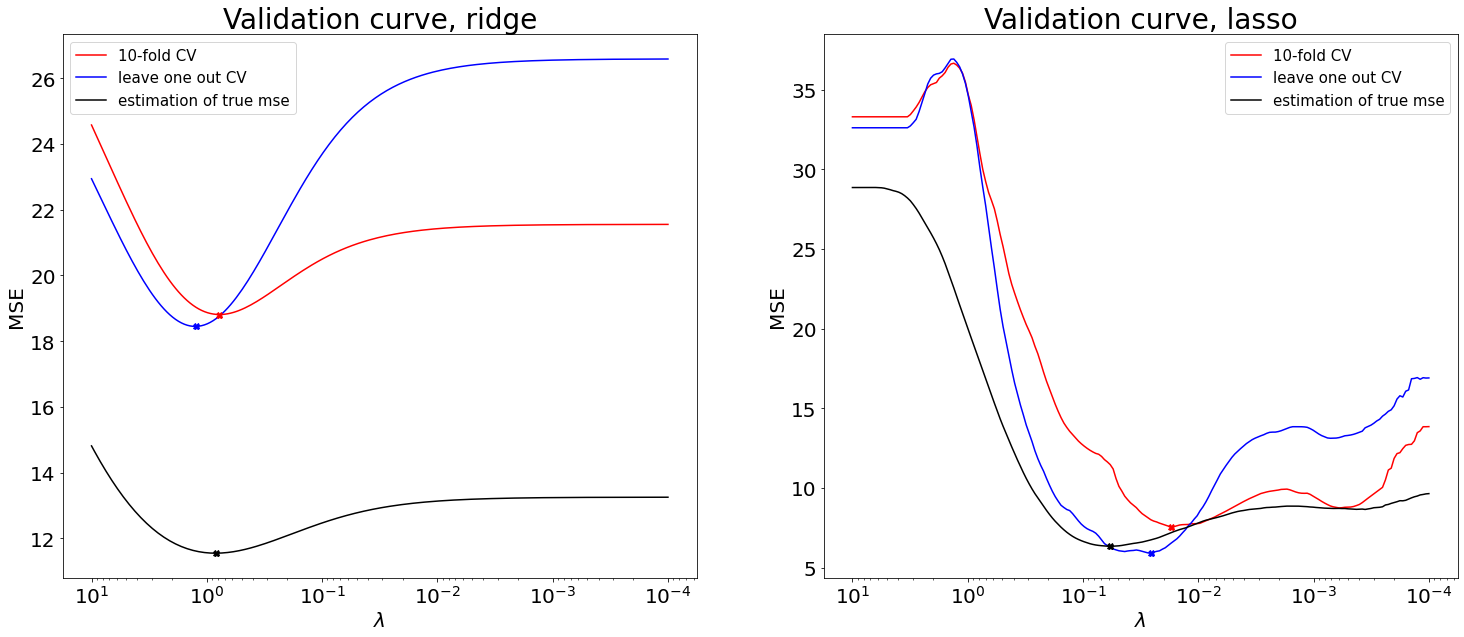
\includegraphics[scale=0.35]{material/Img/CV_simulation.png}
        \centering
        \caption[LOOCV and 10-fold cross-validation comparison]{The LOOCV (blue) and 10-fold cross-validation (blue) comparison for ridge (left) and lasso (right) are depicted above. The approximated true test MSE (black) is also represented. The total number of simulated iterations for each case is $500$.}
        \label{fig:K_LOOOCV}
\end{figure}

\begin{figure}[H]
    %\column{.5\textwidth}
        \centering
        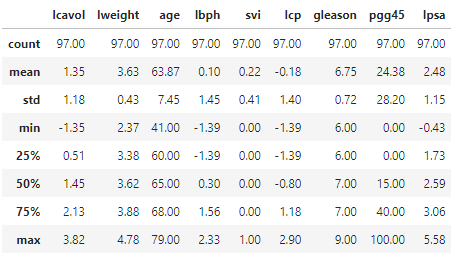
\includegraphics[width=11cm,height=7cm, left]{material/Img/data_descr.png}
        \caption[Data application: descriptive statistics of prostate cancer data set.]{Data application: descriptive statistics of prostate cancer data set.}
        \label{fig:descr_stats}
\end{figure}

\begin{figure}[H]
    %\column{.5\textwidth}
        \centering
        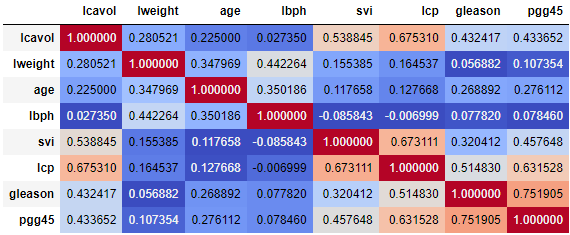
\includegraphics[width=12cm,height=6cm, left]{material/Img/corr_mat_data.png}
        \caption[Data application: correlation matrix]{The correlation matrix of the prostate cancer data set.}
        \label{fig:cor_matr}
\end{figure}

\begin{figure}[H]
\centering
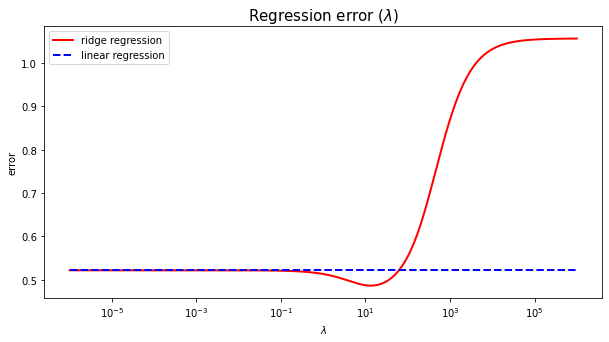
\includegraphics[width=8cm,height=6.5cm, left]{material/Img/data_ridge_vs_lambda.png}
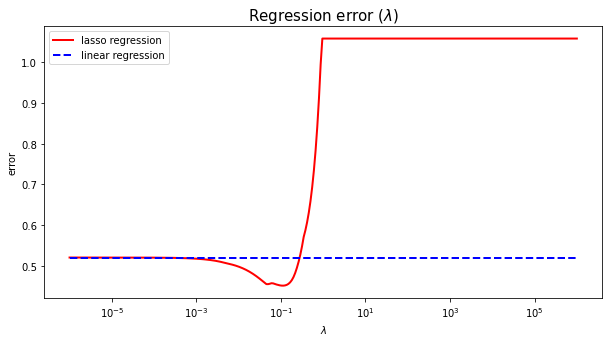
\includegraphics[width=8cm,height=6.5cm, right]{material/Img/data_lasso_vs_lambda.png}\\
%\column{1.0\textwidth}
\centering
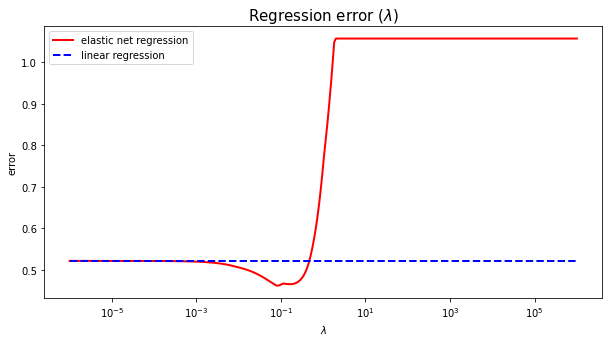
\includegraphics[width=8cm,height=6.5cm, center]{material/Img/data_elnet_vs_lambda.png}\\
\caption[Data application: the MSE path]{Data application: the MSE path. The red curve indicates the regularization method (ridge upper left, lasso upper right, elastic net bottom), and the blue curve indicates the baseline OLS regression.}
 \label{fig:data_mse_path}
\end{figure}

\begin{figure}[H]
\centering
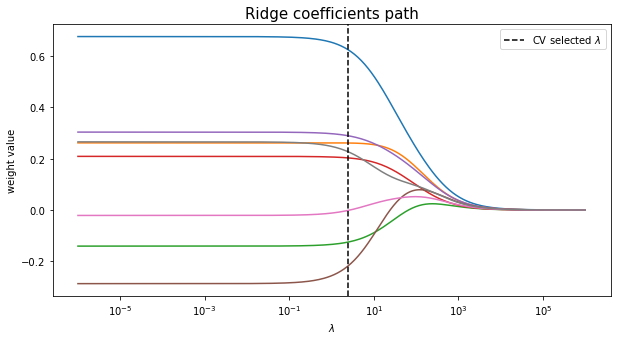
\includegraphics[width=8cm,height=6cm, left]{material/Img/data_ridge_coef_path.png}
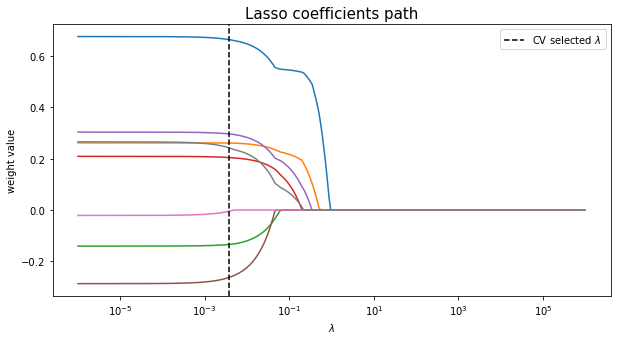
\includegraphics[width=8cm,height=6cm, right]{material/Img/data_lasso_coef_path.png}\\
%\column{1.0\textwidth}
\centering
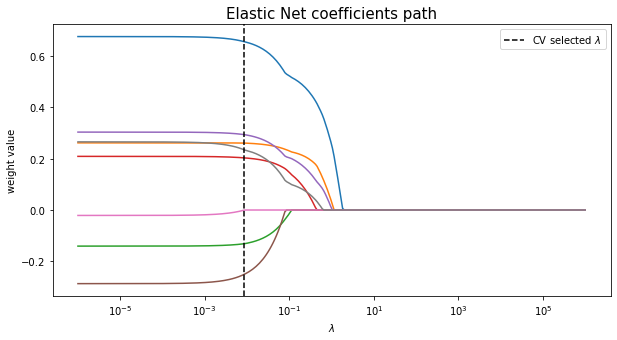
\includegraphics[width=8cm,height=6cm, center]{material/Img/data_elnet_coef_path.png}\\
\caption[Data application: the coefficients path]{Data application: The coefficient paths for the ridge (upper left), lasso (upper right), and naive elastic net (bottom) models are depicted above . The dashed vertical lines indicate the location of the optimally tuned $\lambda$ parameter selected by 10-fold cross-validation.}
\label{fig:data_coef_path}
\end{figure}

\begin{figure}[H]
        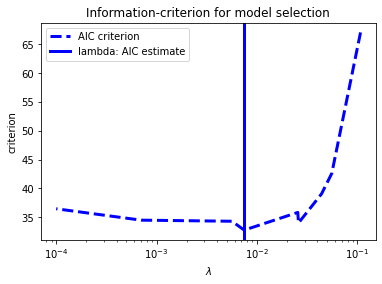
\includegraphics[scale=0.7]{material/Img/AIC_plot.png}%\hspace{-1.2cm}
        \centering
        \caption[Selecting the $\lambda$ tuning parameter via AIC]{The above figure depicts the selection of the $\lambda$ tuning parameter via AIC. The dashed line represent the AIC criterion for each $\lambda$ value after fitting the prostate cancer data set with a LARS model. The vertical line indicates the selected $\lambda$ parameter.}
        \label{fig:AIC}
    \end{figure}

%-------------------- Tables ------------------%%
\subsection{Tables}\label{ap:tables}
% Case 1
\begin{table}[H]
\centering
\begin{tabular}{||c c c c||} 
 \hline
  & High Sparsity & Med. Sparsity & Low Sparsity \\ [0.5ex] 
  Model & $s_0=10$ & $s_0=20$ & $s_0=35$ \\ [0.5ex]
 \hline\hline
 Ridge & 12.544 & 23.895 & \cellcolor{pink!60}36.074\\ 
 \hline
 Elnet (Naive), 0.2 & 10.182 & \cellcolor{pink!60}21.360 & 40.366 \\
 \hline
 Elnet (Naive), 0.5 & 8.760 & 21.687 & 46.961\\
\hline
 Elnet (Naive), 0.7 & 7.421 & 22.380 & 52.046\\
\hline
 Lasso & \cellcolor{pink!60}5.903 & 24.090 & 60.170\\
\hline
\end{tabular}
\caption[Case 1 simulation study]{Case 1 simulation study: set up with $p>n$, $n=30$, $p=35$, and a varying sparsity index $s_{0}$. All truly non-zero beta coefficients have a value of $2$.}
\label{tab:case1}
\end{table}

% Case 2
\begin{table}[H]
\centering
\begin{tabular}{||c c c c||} 
\hline
& High Sparsity & Med. Sparsity & Low Sparsity \\ [0.5ex] 
Model & $s_0=3$ & $s_0=7$ & $s_0=10$ \\ [0.5ex]
\hline\hline
Ridge & 0.570 & 0.270 & \cellcolor{pink!60}1.140 \\
\hline
Elnet (Naive), 0.2 & 0.572 & 0.265 & 1.149 \\
\hline
Elnet (Naive), 0.5 & 0.577 & 0.246 & 1.164\\
\hline
Elnet (Naive), 0.7 & \cellcolor{pink!60}0.552 & \cellcolor{pink!60}0.218 & 1.166\\
\hline
Lasso & 0.607 & 0.298 & 1.166\\
\hline
\end{tabular}
\caption[Case 2 simulation study]{Case 2 simulation study: set up with $p<n$, where $n=30$ and $p=10$, $\rho = 0.8$, and a varying sparsity index $s_{0}$. All truly non-zero beta coefficients are set to $2$. }
\label{tab:case2}
\end{table}

%case3
\begin{table}[H]
\centering
\begin{tabular}{||c c c c||} 
\hline
& Low Pairwise Corr. & Med. Pairwise Corr. & High Pairwise Corr. \\ [0.5ex] 
Model & $\rho=0.1$ & $\rho=0.3$ & $\rho=0.7$\\ [0.5ex]
\hline\hline
Ridge & 1.238 & 2.071 & 0.905\\ 
\hline
Elnet (Naive), 0.2 & 1.160 & 2.034 & 0.889\\
\hline
Elnet (Naive), 0.5 & 0.979 & 1.897 & 0.864\\
\hline
Elnet (Naive), 0.7 & 0.828 & 1.724 & 0.851\\
\hline
Lasso & \cellcolor{pink!60}0.600 & \cellcolor{pink!60}1.340 & \cellcolor{pink!60}0.829\\
\hline
\end{tabular}
\caption[Case 3 simulation study]{Case 3 simulation study: set up with $p<<n$, where $n=20$ and $p=8$, and varying degrees of pairwise correlation, $\rho$. The true beta ceofficients are $\beta \in \{3, 1.5, 0, 0, 2, 0, 0, 0\}$ and therefore reflect a case of high sparsity, where $s_{0}=3$.}
\label{tab:case3}
\end{table}

%Case 4
\begin{table}[H]
\centering
\begin{tabular}{||c c c c||} 
\hline
& Low Pairwise Corr. & Med. Pairwise Corr. & High Pairwise Corr. \\ [0.5ex] 
Model & $\rho=0.1$ & $\rho=0.3$ & $\rho=0.7$\\ [0.5ex]
\hline\hline
Ridge & \cellcolor{pink!60}2.471 & \cellcolor{pink!60}0.521 & \cellcolor{pink!60}0.736\\ 
\hline
Elnet (Naive), 0.2 & 2.506 & 0.585 & 0.772\\
\hline
Elnet (Naive), 0.5 & 2.542 & 0.882 & 0.831\\
\hline
Elnet (Naive), 0.7 & 2.548 & 1.124 & 0.867\\
\hline
Lasso & 2.548 & 1.532 & 0.906\\
\hline
\end{tabular}
\caption[Case 4 simulation study]{Case 4 simulation study: set up with $p<<n$, where $n=30$ and $p=8$, and varying degrees of pairwise correlation, $\rho$. All beta coefficients are non-zero with a value of $0.85$, indicating no sparsity.}
\label{tab:case4}
\end{table}

%case5
\begin{table}[H]
\centering
\begin{tabular}{||c c c c||} 
\hline
& Low Pairwise Corr. & Med. Pairwise Corr. & High Pairwise Corr. \\ [0.5ex] 
Model & $\rho=0.1$ & $\rho=0.3$ & $\rho=0.7$\\ [0.5ex]
\hline\hline
Ridge & 9.412 & 15.714 & 3.263\\ 
\hline
Elnet (Naive), 0.2 & 7.932 & 11.092 & 2.659\\
\hline
Elnet (Naive), 0.5 & 6.049 & 10.505 & 1.882\\
\hline
Elnet (Naive), 0.7 & 5.122 & 8.570 & \cellcolor{pink!60}1.589 \\
\hline
Lasso & \cellcolor{pink!60}4.079 & \cellcolor{pink!60}6.575 & 1.716 \\
\hline
\end{tabular}
\caption[Case 5 simulation study]{Case 5 simulation study: set up with $p>n$, where $n=30$ and $p=35$, high sparsity ($s_0=10$), and varying degrees of pairwise correlation, $\rho$. All truly non-zero beta coefficients have a value of $2$.}
\label{tab:case5}
\end{table}

\begin{table}[H]
\centering
\begin{tabular}{||c c c c c c c||} 
 \hline
  & Linear & Ridge & Lasso & Naive Elastic Net & LARS  & LARS  \\ [0.5ex] 
  Coefficients & & & & & \emph{(AIC)} & \emph{(10-fold CV)}\\ [0.5ex]
 \hline\hline
 lcavol & 0.676 & 0.624 & 0.664 & 0.624 & 0.547 & 0.662\\
 \hline
 lweight & 0.262 &  0.261 & 0.261 & 0.261 &  0.220 & 0.261\\
 \hline
 age & -0.141 & -0.125 & -0.134 & -0.125 & - & -0.133\\
\hline
 lbph & 0.209 & 0.203 & 0.205 & 0.203 & 0.142 & 0.203\\
\hline
 svi & 0.304 & 0.289 & 0.297 & 0.289 & 0.196 & 0.295\\
\hline
 lcp & -0.287 & -0.216 & -0.263 & -0.216 & - & -0.258\\
 \hline
 gleason & -0.021 & -0.001 & -0.005 & -0.001 & - & -0.002\\
 \hline
 pgg45 & 0.266 & 0.226 & 0.243 & 0.226 & 0.086 & 0.237\\
 \hline
\end{tabular}
\caption[Data application: table of estimated coefficients for all fitted models]{Data application: table of estimated coefficients for all fitted models.}
\label{tab:coef_table}
\end{table}

    
\begin{table}[H]
\centering
\begin{tabular}{||c c c c||} 
 \hline
 Model & Test MSE (with 10-fold CV) & Test MSE (AIC) & Variable Selection\\ [0.5ex] 
 \hline\hline
 Linear & 0.5213 & - & All\\ 
 \hline
 Ridge & 0.5043 & - & All\\
 \hline
 Lasso coordinate descent & 0.5112 & - & All\\
 \hline
 Elastic Net (Naive) & 0.5043 & - & All\\
 \hline
  Lasso LARS & 0.5084 & - & All\\
 \hline
 Lasso LARS & - & 0.5033 & lcavol, lweight, lbph, \\ & & & svi, pgg45\\
 \hline
\end{tabular}
\caption[Data application: model selection]{The above table outlines the prediction performance of all models fitted to the prostate cancer data set.}
\label{tab:mod_sel}
\end{table}

%-------------CV-Simulation----------------%
\subsection{Cross-validation robustness check}
\label{section:cvsim}

\noindent According to \cite{james2013introduction}, cross-validation is a valuable method for calculating the test error rate for each $\lambda$ in the predetermined grid of the tuning parameter values. We can then choose the $\lambda$ value that minimizes the prediction error of the test set. In a real data setting, we refit the model(s) using all observations in our original data set as well as the chosen tuning parameter.  \\    

\noindent This simulation depicted in Figure \ref{fig:K_LOOOCV} compares the accuracy of the LOOCV and 10-fold cross-validation procedures with an estimate of the true MSE over a range of $\lambda$ tuning parameters for ridge and lasso, respectively. We employ a simple high-dimensional data setup with $30$ observations, $10$ non-zero coefficients that have a magnitude of $2$, and $25$ truly zero coefficient estimates. We do not include any pairwise correlation among regressors. The approximation of the true test MSE is computed using the same procedure as above to compute the test MSEs for a comparison of each regularization method's goodness-of-fit based on $500$ randomly selected data sets. In both plots of Figure \ref{fig:K_LOOOCV}, the approximated true test MSE is represented by black curves, while the LOOCV and 10-fold cross-validation estimates are characterized by the blue and red curves, respectively. While the cross-validation estimates in both plots exhibit a similar shape to the estimation of the true test MSE, it is apparent, particularly in the first graph, that the cross-validation curves overestimate the approximation of the true MSE. However, \cite{james2013introduction} indicate that the location of the minimized test error may be of greater interest than the actual estimated value of the test MSE derived through cross-validation.  \\

\noindent In the context of regularized regression, this important distinction between the actual value that minimizes the test error and the location of this value holds true: when evaluating which cross-validation method proves most suitable for selecting the optimal value of the tuning parameter, we are more concerned with the location of the minimum as opposed to the size of the test MS itself. As depicted in the test MSE curves computed for our simulation exercise, the LOOCV as well as the 10-fold cross-validation method suitably approximate the location of the minimized test error such that either procedure will yield an appropriate estimate of the optimal $\lambda$ tuning parameter. It is important to note for this simulation exercise, however, that we do not vary the setup of our randomly sampled data sets to confirm the robustness of our results in the case of lower degrees of sparsity and/or pairwise correlation among regressors.    

%------------------ Proofs---------------------%
\subsection{Proofs}\label{proofs}

For the proofs to derive the beta estimator, bias, and variance of ridge regression, we assume that the matrix $\mathbf{X}$ has full rank such that the OLS estimator $\hat{\beta}_{OLS}=(\mathbf{X}^{\prime} \mathbf{X})^{-1} \mathbf{X}^{\prime} \mathbf{Y}$ exists. We also assume exogeneity, $\mathbf{E}(\varepsilon)=0$, and spherical errors, $\operatorname{Var}(\hat{\beta}_{OLS})=\sigma^2(\mathbf{X}^{\prime} \mathbf{X})^{-1} $. 

\subsubsection{Ridge estimator}\label{proof:ridgeestimate}

\noindent The ridge minimization problem can be expressed in matrix notation as follows:
\begin{align*}
& \operatorname{RSS} + \lambda \beta^{\prime} \beta \\
& (\mathbf{y} - \mathbf{X}\beta)^{\prime}(\mathbf{y} - \mathbf{X}\beta) + \lambda \beta^{\prime}\beta \\
& \mathbf{y^{\prime}} \mathbf{y} -2\beta^{\prime}\mathbf{X}^{\prime}\mathbf{y} + \beta^{\prime}\mathbf{X}^{\prime}\mathbf{X}\beta + \lambda \beta^{\prime}\beta
\end{align*}

\noindent Taking the derivative with respect to $\beta$ and solving for $\beta$, we get:

\begin{align*}
 \frac{\partial}{\partial \beta} = -2 \mathbf{X}\mathbf{y} + 2 \mathbf{X}^{\prime}\mathbf{X}\beta + 2\lambda\beta &=0 \\
-\mathbf{X}\mathbf{y} +  \mathbf{X}^{\prime} \mathbf{X} + \lambda\beta&=0 \\
\mathbf{X}^{\prime} \mathbf{X}\beta+\lambda\beta&= \mathbf{X}^{\prime} \mathbf{y} \\
\hat{\beta}^{R}&= (\mathbf{X}^{\prime} \mathbf{X} + \lambda \mathbf{I})^{-1} \mathbf{X}^{\prime} \mathbf{y}
\end{align*}

%-----------------------------------------------
\subsubsection{Bias of ridge estimator} \label{proofbias}

Following \cite{van2015lecture}, take the expectation of the ridge estimator:
\begin{align*}
\mathbf{E}\left[\hat{\beta}^{R}\right] &=\mathbf{E}\left[\left(\mathbf{X}^{\prime} \mathbf{X}+\lambda \mathbf{I}\right)^{-1} \mathbf{X}^{\prime} \mathbf{y}\right]\\
&=\mathbf{E}\left[\left(\mathbf{X}^{\prime} \mathbf{X}+\lambda \mathbf{I}\right)^{-1} \mathbf{X}^{\prime} (\mathbf{X}\beta - \varepsilon)\right]\\
&=\mathbf{E}\left[\left(\mathbf{X}^{\prime} \mathbf{X}+\lambda \mathbf{I}\right)^{-1} \mathbf{X}^{\prime} \mathbf{X} \beta - \mathbf{X}^{\prime} \varepsilon)\right]\\
&=\left(\mathbf{X}^{\prime} \mathbf{X}+\lambda \mathbf{I}\right)^{-1} \mathbf{X}^{\prime} \mathbf{X} \beta - \mathbf{X}^{\prime} \mathbf{E}(\varepsilon)\\
&=\left(\mathbf{X}^{\prime} \mathbf{X}+\lambda \mathbf{I}\right)^{-1} \mathbf{X}^{\prime} \mathbf{X} \beta,
\end{align*}

\noindent where $\mathbf{E}\left[\hat{\boldsymbol{\beta}}^{R}\right] \neq \beta$ for any $\lambda >0$. Hence, the ridge estimator is unbiased $\mathbf{iff}$ $\lambda=0$ such that $\hat{\beta}^R=\hat{\beta}_{OLS}$. The extent of the bias is:

\begin{align*}
\mathbf{E}\left[\hat{\beta}^{R}\right] - \beta=\left(\mathbf{X}^{\prime} \mathbf{X}+\lambda \mathbf{I}\right)^{-1} \mathbf{X}^{\prime} \mathbf{X} \beta - \beta
\end{align*}

%-------------------------------------------------
\subsubsection{Variance of ridge estimator} \label{proofvar}
Following \cite{van2015lecture}, when the matrix $\mathbf{X}$ has full rank, there is a linear relationship between ridge and its maximum likelihood estimator. We can define the linear operator as $\mathbf{W}_\lambda=\left(\mathbf{X}^{\prime} \mathbf{X}+\lambda \mathbf{I}\right)^{-1} \mathbf{X}^{\prime} \mathbf{X}$. The ridge estimator can be expressed as $\mathbf{W}_\lambda \hat{\beta}_{OLS}$:

\begin{align*}
\mathbf{W}_{\lambda} \hat{\beta}_{OLS} &=\mathbf{W}_{\lambda}\left(\mathbf{X}^{\prime} \mathbf{X}\right)^{-1} \mathbf{X}^{\prime} \mathbf{y} \\
&=\left(\mathbf{X}^{\prime} \mathbf{X}+\lambda \mathbf{I}\right)^{-1} \mathbf{X}^{\prime} \mathbf{X}\left(\mathbf{X}^{\prime} \mathbf{X}\right)^{-1} \mathbf{X}^{\prime} \mathbf{Y} \\
&=\left(\mathbf{X}^{\prime} \mathbf{X}+\lambda \mathbf{I}\right)^{-1} \mathbf{X}^{\prime} \mathbf{y} \\
&=\hat{\beta}^{R},
\end{align*}

\noindent where $\mathbf{W}_{\lambda}$ is a non-random matrix. We can use this property to show the variance of the ridge estimator:

\begin{align*}
\operatorname{Var}\left[\hat{\beta}^{R}\right]&=\operatorname{Var}\left[\mathbf{W}_\lambda\hat{\beta}_{OLS}\right]\\
&=\mathbf{W}_{\lambda}\operatorname{Var}\left[\hat{\beta}_{OLS}\right]\mathbf{W}_{\lambda}^{\prime}\\
&=\sigma^2 \mathbf{W}_\lambda (\mathbf{X}^{\prime} \mathbf{X})^{-1}\mathbf{W}_{\lambda}^{\prime}\\
&=\sigma^2\left(\mathbf{X}^{\prime} \mathbf{X}+\lambda \mathbf{I}\right)^{-1}(\mathbf{X}^{\prime} \mathbf{X})\left(\mathbf{X}^{\prime} \mathbf{X}+\lambda \mathbf{I}\right)^{-1}
\end{align*}

\noindent We can now compare the variance of the ridge and OLS estimators:

\begin{align*}
\operatorname{Var}[\hat{\beta}_{OLS}]-\operatorname{Var}[\hat{\beta}^{R}] &= \sigma^{2}(\mathbf{X}^{\prime} \mathbf{X})^{-1} - \sigma^2 \mathbf{W}_\lambda (\mathbf{X}^{\prime}\mathbf{X})^{-1}\mathbf{W}_{\lambda}^{\prime}\\
&=\sigma^{2}\left[\left(\mathbf{X}^{\prime} \mathbf{X}\right)^{-1}-\mathbf{W}_{\lambda}\left(\mathbf{X}^{\top} \mathbf{X}\right)^{-1} \mathbf{W}_{\lambda}^{\prime}\right] \\
&=\sigma^{2} \mathbf{W}_{\lambda}\left\{\left[\mathbf{I}+\lambda\left(\mathbf{X}^{\prime} \mathbf{X}\right)^{-1}\right]\left(\mathbf{X}^{\prime} \mathbf{X}\right)^{-1}\left[\mathbf{I}+\lambda\left(\mathbf{X}^{\prime} \mathbf{X}\right)^{-1}\right]^{\prime}-\left(\mathbf{X}^{\prime} \mathbf{X}\right)^{-1}\right\} \mathbf{W}_{\lambda}^{\prime} \\
&=\sigma^{2} \mathbf{W}_{\lambda}\left[2 \lambda\left(\mathbf{X}^{\prime} \mathbf{X}\right)^{-2}+\lambda^{2}\left(\mathbf{X}^{\prime} \mathbf{X}\right)^{-3}\right] \mathbf{W}_{\lambda}^{\prime} \\
&=\sigma^{2}\left(\mathbf{X}^{\top} \mathbf{X}+\lambda \mathbf{I}\right)^{-1}\left[2 \lambda \mathbf{I}+\lambda^{2}\left(\mathbf{X}^{\prime} \mathbf{X}\right)^{-1}\right]\left[\left(\mathbf{X}^{\prime} \mathbf{X}+\lambda \mathbf{I}\right)^{-1}\right]^{\prime}
\end{align*}

\noindent Since each component in the matrix product is non-negative definite, the difference between the variances is also non-negative definite. This means that the variance of the OLS estimator is larger than the variance of the ridge estimator.

%-------------------------------------------------
% \subsubsection{Centering condition for the intercept}
% \noindent Solving for $\beta_0$ from the following optimization problem gives the following first order condition: 

% $$
% \begin{aligned}
% \frac{d}{d\beta}(\sum_{i=1}^{N}(y_i-\beta_0-\sum_{j}\beta_j x_{i})^2=0 \\
% \sum_{i=1}^{N}2(y_i-\beta_0-\sum_{j}\beta_j x_{i})=0 \\
% \sum_{i=1}^{N}y_i-N\beta_0-\sum_{i,j}\beta_j x_{i,j}=0, \\
% \end{aligned}
% $$

% \noindent where
% $$
% \sum_{i,j}\beta_j x_{i,j}=0
% $$

% \noindent and

% $$
% \beta_0=\frac{1}{N}\sum_{i=1}^{N}y_i.
% $$


%--------------------------------------------------
\subsubsection{Lasso subgradient solution}
\label{subgradient}

\noindent Considering the following multivariate regression without an intercept:

\begin{align*}
Y_{i}= \beta_j X_{ij} +\varepsilon_{i} 
\end{align*}

\noindent  where the residual is:

\begin{align*}
\hat{\varepsilon}_i=Y_i - \hat{Y_i}=Y_i - \hat{\beta}_j X_{ij}
\end{align*}

\noindent We derive the OLS estimate algebraically by minimizing the RSS with respect to $\beta_j$:

\begin{align*}
\operatorname{RSS}&=\sum_{i=1}^{n}\varepsilon_i^2 \\
&= \sum_{i=1}^{n}(Y_{i} -\beta_j X_{ij})^2 \\
%\frac{\partial}{\partial w_{j}} %\operatorname{RSS}(\mathbf{w})=a_{j} w_{j}-c_{j}
\end{align*}
Solving for the partial derivative with respect to $\beta_j$ we get:

\begin{align*}
   \frac{\partial \operatorname{RSS}}{\partial \beta_{j}}=2\sum_{i=1}^{n}\left(\beta_{j} X_{ij}^{2}- Y_{i} X_{ij}\right) 
\end{align*}

\noindent From this point, we closely follow the derivation presented in \cite{murphy2012machine}. Let us reformulate slightly the non-regularized RSS such that we also take into account the correlation between the $j$th regressor and the residual: 

\begin{align*}
\frac{\partial}{\partial \beta_{j}} \operatorname{RSS}(\mathbf{\beta}) &=a_{j} \beta_{j}-c_{j} \\
a_{j} &=2 \sum_{i=1}^{n} x_{i j}^{2} \\
c_{j} &=2 \sum_{i=1}^{n} x_{i j}\left(y_{i}-\mathbf{\beta}_{-j}^{T} \mathbf{x}_{i,-j}\right)
\end{align*}

\noindent where $c_j$ is the correlation between the $j$'th regressor and the residual conditioned on all other regressors, $\mathbf{r}_{-j}=\mathbf{y}-\mathbf{X}_{:,-j} \mathbf{\beta}_{-j}$. Consider now the following formulation of the lasso problem by adding the penalty term that, as expressed in Section \ref{section:lasso}, is a non-smooth function. 

\begin{align*}
f(\beta)=\operatorname{RSS}(\beta)+\lambda\|\mathrm{\beta}\|_{1}
\end{align*}

\noindent This is a non-smooth function with a kink at $\beta_{j}=0$, and thus we need to define subgradients (or subderivatives) at $\beta_{j}=0$. The subderivatives for the lasso problem are:
\begin{align*}
\partial_{\beta_{j}} f(\mathbf{\beta}) &=\left(a_{j} \beta_{j}-c_{j}\right)+\lambda \partial_{\beta_{j}}\|\mathbf{\beta}\|_{1} \\
&=\left\{\begin{array}{cl}
\left\{a_{j} \beta_{j}-c_{j}-\lambda\right\} & \text { if } \beta_{j}<0 \\
{\left[-c_{j}-\lambda,-c_{j}+\lambda\right]} & \text { if } \beta_{j}=0 \\
\left\{a_{j} \beta_{j}-c_{j}+\lambda\right\} & \text { if } \beta_{j}>0
\end{array}\right.
\end{align*}

\noindent The first and third case correspond to points where the function is differentiable and its derivative is expressed as a set with one element (i.e., as a singleton). The second case, however, is the case for which the function's derivative is not well defined. Here, the subderivative is expressed as an interval. Depending on the magnitude of $c_j$, it is possible for the solution $\partial_{\beta_{j}} f(\mathbf{\beta})=0$ to occur at 3 different values of $\beta_j$, and thus, we can trace the lasso estimates as follows:

\begin{align*}
\hat{\beta}_{j}\left(c_{j}\right)=\left\{\begin{array}{cc}\left(c_{j}+\lambda\right) / a_{j} & \text { if } c_{j}<-\lambda \\ 0 & \text { if } c_{j} \in[-\lambda, \lambda] \\ \left(c_{j}-\lambda\right) / a_{j} & \text { if } c_{j}>\lambda\end{array}\right.
\end{align*}

\noindent where, given a sufficiently small $c_j$ or a sufficiently large $\lambda$, the $j$th coefficient will be set to zero by the lasso. \\

\noindent The solution can be re-written as pointed out by the authors:

\begin{align*}
    \hat{\beta}_{j}=\operatorname{soft}\left(\frac{c_{j}}{a_{j}} ; \frac{\lambda}{a_{j}}\right)
\end{align*}

%-------------------- Algo ------------------%%
\subsection{Lasso algorithms}\label{algorithms}

\subsubsection{Coordinate descent for lasso}

\noindent The notation for the coordinate descent lasso algorithm is based on \cite{murphy2012machine} and follows the notation outlined in Section \ref{subgradient}.

\begin{algorithm}[H]
\caption{Coordinate descent for lasso}\label{alg:1}
1. Initialize $\mathbf{\beta}=\left(\mathbf{X}^{\prime} \mathbf{X}+\lambda \mathbf{I}\right)^{-1} \mathbf{X}^{\prime} \mathbf{y}$. \\
2. For $j=1,...,p$: 
\begin{enumerate}
    \  $a_{j}=2 \sum_{i=1}^{n} x_{i j}^{2}$ \\
    \  $c_{j}=2 \sum_{i=1}^{n} x_{i j}\left(y_{i}-\mathbf{w}^{T} \mathbf{x}_{i}+w_{j} x_{i j}\right)$ \\
    \  $w_{j}=\operatorname{soft}\left(\frac{c_{j}}{a_{j}}, \frac{\lambda}{a_{j}}\right)$
\end{enumerate}
3. Repeat step (2) many times until \textit{converged}.
\end{algorithm}

\subsubsection{Least angle regression and shrinkage (LARS)}
\noindent Following \cite{hastie2008elements}:

\begin{algorithm}[H]
\caption{LARS}\label{alg:2}
1. Initialize with residual $\mathbf{r}=\mathbf{y}-\overline{\mathbf{y}}$ and a large enough $\lambda$. \\
2. Find regressor $x_{ij}$ most correlated with the residual. \\
3. Decrease $\lambda$ until another regressor $x_{i,-j}$ has as much correlation with $\mathbf{r}$ as $x_{ij}$. \\
4. If a non-zero coefficient hits zero, \textbf{drop variable from the active set}
of variables and recompute the current joint least squares direction.\\
4. Repeat (2) and (3) for all $p$ predictors.

\end{algorithm}

%------------------ AIC---------------------%
\subsection{Akaike information criterion (AIC)}

\noindent The Akaike information criterion (AIC) \citep{akaike1974new} is an estimator of out-of-sample prediction error and thereby serves as an indicator for the relative quality of a statistical model. Given a collection of models, AIC estimates the quality of each model relative to the others. Thus, AIC provides a means for model selection. AIC uses a model’s maximum likelihood estimation (i.e., log-likelihood) as a measure of fit. AIC works by evaluating the model’s fit on the training data and adding a penalty term relative to the complexity of the model. The desired result is to find the lowest possible AIC, which indicates the best balance of model fit with generalizability.\\

\noindent Let $d$ be the number of estimated parameters in the model and $\hat{L}$ be the maximum value of the likelihood function for the model. Then the AIC value of the model is:

\begin{equation}
\mathrm{AIC}=2 d-2 \ln (\hat{L})
\end{equation}

\noindent Thus, AIC rewards goodness of fit (as assessed by the likelihood function), but it also includes a penalty that is an increasing function of the number of estimated parameters.\\

\noindent An alternative formula for least-squares-regression-type analyses with normally distributed errors is:

\begin{equation}
\mathrm{AIC}=\frac{1}{n \hat{\sigma}^{2}}\left(\mathrm{RSS}+2 d \hat{ \sigma}^{2}\right) ,
\end{equation}

\noindent where $\hat{\sigma}^{2}$ is an estimate of the variance error, $\epsilon$.


%------------------ scikit---------------------%
\subsection{Software computation}\label{section:software}

\noindent According to the scikit-learn documentation, the ridge minimization problem is:

\begin{equation}
\label{eqn:ridge_scikit}
\underset{\beta}{\operatorname{min}} \|y-\mathbf{X}\beta\|_{2}^{2} + \lambda\|\beta\|_{2}^{2} \end{equation}
Similarly, the elastic net minimization problem is:
\begin{equation}
\label{eqn:elnet_scikit}
\underset{\beta}{\operatorname{min}} \frac{1}{2n}\|y-\mathbf{X}\beta\|_{2}^{2} + \lambda\alpha\|\beta\|_{1} + \frac{\lambda(1-\alpha)}{2}\|\beta\|_{2}^{2},   
\end{equation}

\noindent where $\alpha$ is the $\ell_1$-ratio and $\lambda$ is the model's shrinkage penalty.\\

\noindent There are two important facts to note about the scikit-learn package. First, the minimization problem in equation \eqref{eqn:elnet_scikit} follows the same structure as equation \eqref{eqn:eqn8}. Therefore, scikit-learn computes only the naive elastic net. Second, when the $\ell_1$-ratio is 0 (i.e., ridge) the minimization problem in equation \eqref{eqn:elnet_scikit} simplifies to
$\Big\{\underset{\beta}{\operatorname{min}} \frac{1}{2n}\|y-\mathbf{X}\beta\|_{2}^{2} +  \frac{\lambda}{2}\|\beta\|_{2}^{2}\Big\}$, which does not exactly match equation \eqref{eqn:ridge_scikit}. This can explain the reason why in our data application the two computations return different optimal values for the $\lambda$ tuning parameter.\footnote{For further details, refer to the scikit-learn documentation for \href{https://scikit-learn.org/stable/modules/generated/sklearn.linear_model.Ridge.html}{ridge} and \href{https://scikit-learn.org/stable/modules/generated/sklearn.linear_model.ElasticNet.html}{elastic net}.}







